% Applied Sciences (MDPI) manuscript — Lite AIGC Detect
% Compile from this directory: pdflatex main && bibtex main && pdflatex main && pdflatex main
% Requires: Definitions/ (official MDPI class), figures/
% Support: latex@mdpi.com
%=================================================================
\documentclass[applsci,article,submit,pdftex,moreauthors]{Definitions/mdpi}

%=================================================================
\firstpage{1}
\makeatletter
\setcounter{page}{\@firstpage}
\makeatother
\pubvolume{1}
\issuenum{1}
\articlenumber{0}
\pubyear{2026}
\copyrightyear{2026}
\datereceived{ }
\daterevised{ }
\dateaccepted{ }
\datepublished{ }
\hreflink{https://doi.org/}

% tabularx right-aligned X column used in result tables
\newcolumntype{R}{>{\raggedleft\arraybackslash}X}

%=================================================================
\Title{Lightweight AI-Generated Image Detection under Compression and Cross-Generator Shift: A Reproducible Study of CNN, Frequency-Aware, and State-Space Models}

\TitleCitation{Lightweight AI-Generated Image Detection under Compression and Cross-Generator Shift}

% Author metadata (single author for current submission; co-authors may be added later)
\newcommand{\orcidauthorA}{0009-0001-4945-6733}

\Author{Kaihao Chen $^{1}$\orcidA{}$^{*}$}

\AuthorNames{Kaihao Chen}

\isAPAStyle{%
       \AuthorCitation{Chen, K.}
         }{%
        \isChicagoStyle{%
        \AuthorCitation{Chen, Kaihao.}
        }{
        \AuthorCitation{Chen, K.}
        }
}

\address{%
$^{1}$ \quad College of Software Engineering, South China Agricultural University, Guangzhou, Guangdong, China; 13543148496@163.com}

\corres{Correspondence: 13543148496@163.com}

% Structured abstract without headings (MDPI style); keep $\approx$200 words
\abstract{Background: Deployable AI-generated still-image detectors must balance accuracy with efficiency under compression and generator shift, yet many comparisons mix training protocols or rely on pretrained backbones. Methods: We compare compact CNNs, a gated frequency-aware CNN (LiteFreqNet~v2), and two study-specific pure-PyTorch state-space classifiers (\textbf{LiteSSM-A} and \textbf{LiteSSM-B}) trained from scratch under a locked recipe on DiffusionForensics (ADM bedroom + SDv2 CelebA-HQ). Models are selected by validation AUC and evaluated with Params/FLOPs, locked batch-1 latency, batch-32 throughput, JPEG Q70, content-domain splits, and UniversalFakeDetect (UFD) per-generator scores. Public UnivFD and NPR checkpoints provide a separate pretrained reference panel. We treat UFD Macro AUC as the primary cross-generator metric. Results: Among protocol-matched compact models, LiteSSM-A attains the highest UFD Macro (0.718; ID 0.946; bedroom $\approx$0.81) at 1.74M parameters, with locked batch-1 p50 latency 144.4\,ms and batch-32 throughput 226 images/s (FP32, RTX~4090D); pretrained references reach higher absolute Macro (UnivFD 0.948; NPR 0.976) under different training paradigms. DALL·E remains near chance for all Panel~A models; JPEG Q70 changes AUC by at most 0.003; frequency modules are not universally helpful. Conclusions: LiteSSM-A is the preferred generalization--efficiency operating point within the studied lightweight protocol, while generator- and domain-specific boundaries preclude overgeneralized detection claims.}

\keyword{AI-generated image detection; lightweight neural networks; state-space models; frequency features; out-of-distribution generalization; JPEG compression; reproducible benchmarking}

% Optional for Applied Sciences
\featuredapplication{Compact still-image AIGC screening on GPU servers where parameter count, throughput, JPEG stability, and honest cross-generator failure reporting matter more than peak in-distribution accuracy alone.}

\begin{document}

%%%%%%%%%%%%%%%%%%%%%%%%%%%%%%%%%%%%%%%%%%
\section{Introduction}
\label{sec:introduction}
Synthetic still images from modern generative models are increasingly difficult to separate from photographs by casual inspection, yet many content-moderation pipelines must run under tight latency and parameter budgets.
The practical question is therefore not only which architecture maximizes in-distribution (ID) accuracy, but which compact detector offers a usable accuracy--efficiency trade-off once images leave the training generators and pass through ordinary recompression.

Prior work has explored CNN detectors~\cite{wang2020cnn,tan2019efficientnet}, frequency-domain cues~\cite{frank2020freq}, and, more recently, state-space sequence models~\cite{gu2023mamba}.
Reported gains are often entangled with mismatched training protocols, ImageNet initialization, or heterogeneous evaluation sets, which complicates deployment decisions.
Frequency features are sometimes presented as broadly helpful for diffusion artifacts; likewise, strong ID scores can conceal fragile transfer to particular generators or content domains~\cite{ojha2023ufd}.

This paper contributes a \emph{protocol-locked empirical study} rather than a claim of state-of-the-art accuracy.
Under a single no-pretraining recipe, we compare:
\begin{enumerate}
\item compact CNN baselines (EfficientNet-B0, MobileNetV3-Small, ShuffleNetV2-x0.5)~\cite{tan2019efficientnet,howard2019mobilenetv3,ma2018shufflenet};
\item a gated frequency-aware CNN (LiteFreqNet~v2) and related ablations;
\item two study-specific pure-PyTorch SSM classifiers (\textbf{LiteSSM-A} and \textbf{LiteSSM-B}), with and without an attached frequency branch.
\end{enumerate}

Evaluation covers ID test performance, content-domain splits (CelebA-HQ vs.\ bedroom), UniversalFakeDetect (UFD) per-generator and Macro averages~\cite{ojha2023ufd}, JPEG quality-70 recompression, and measured efficiency (parameters, FLOPs, batch-1 latency, batch-32 throughput).
External pretrained reference detectors (UnivFD, NPR) are reported in a separate panel for contextualization only~\cite{ojha2023ufd,tan2024npr}.
An unmatched FLUX probe is deferred to the appendix and is not used for architecture claims~\cite{flux2024}.
We explicitly separate \textbf{UFD Macro AUC} from \textbf{OOD Pooled AUC} to avoid metric ambiguity.

\paragraph{Main finding.}
Under the evaluated latency budget, \textbf{LiteSSM-A} is the recommended compact operating point in the training-matched panel, improving average cross-generator behavior relative to the CNN suite, but \emph{no evaluated model}---including SSMs---removes generator-specific failures (notably DALL·E) or content-domain difficulty (bedroom).
Frequency enhancement is not universally beneficial under our protocol.

The remainder of the paper is organized as follows.
Section~\ref{sec:related} situates related detectors.
Section~\ref{sec:methods} details data, training, metrics, and reproducibility controls.
Section~\ref{sec:results} reports results.
Section~\ref{sec:discussion} discusses metric definitions, deployment implications, and boundaries.
Section~\ref{sec:conclusions} concludes.


%%%%%%%%%%%%%%%%%%%%%%%%%%%%%%%%%%%%%%%%%%
\section{Related Work}
\label{sec:related}
\subsection{CNN and Artifact-Based Detection}
\label{sec:rw-cnn}

CNN-based detectors remain the dominant practical baseline for still-image real/fake classification.
Early work showed that CNN-generated images leave transferable forensic cues that a ResNet-style classifier can exploit across several GAN families~\cite{wang2020cnn}.
Subsequent studies emphasized local texture, upsampling footprints, and neighboring-pixel dependencies as more stable signals than global semantics alone.
In particular, Neighboring Pixel Relationships (NPR) treat the local interdependence induced by generator upsampling operators as a transferable artifact representation and report strong cross-generator behavior under their official training and evaluation protocol~\cite{tan2024npr}.
We treat NPR as an \emph{external pretrained reference} rather than a training-matched competitor: its native preprocessing and released weights are used for inference-only contextualization on our frozen manifests.

Compact ImageNet-style backbones (EfficientNet, MobileNet, ShuffleNet) are widely used when parameter count and throughput matter~\cite{tan2019efficientnet,howard2019mobilenetv3,ma2018shufflenet}.
In this study they form the controlled lightweight CNN panel trained from scratch under a locked recipe.

\subsection{Pretrained and CLIP-Based Universal Detectors}
\label{sec:rw-univfd}

A complementary line of work avoids learning a heavily tuned ``fake'' detector and instead probes large pretrained feature spaces.
UniversalFakeDetect (UnivFD) uses frozen CLIP ViT-L/14 features with a linear probe (or nearest-neighbor variants) and demonstrates improved transfer to unseen generative families relative to detectors trained end-to-end on a single generator breed~\cite{ojha2023ufd}.
The strength of this approach is precisely its large-scale pretraining; therefore UnivFD is \emph{not} comparable under an identical from-scratch lightweight protocol.
We include the publicly released UnivFD checkpoint as a second external reference panel to situate our compact models, while keeping Panel~A (training-matched) and Panel~B (pretrained references) separate in the results tables.

\subsection{Diffusion-Specific and Reconstruction-Based Detection}
\label{sec:rw-dire}

Diffusion-oriented detectors often exploit reconstruction error or diffusion-specific representations.
DIRE distinguishes real and generated images via the discrepancy between an input and its diffusion reconstruction~\cite{wang2023dire}.
Such pipelines can improve robustness on diffusion imagery, but they introduce a heavy generative-model reconstruction stage that differs from the lightweight direct-classification deployment target studied here.
We therefore discuss DIRE and related reconstruction approaches as literature context and do \emph{not} re-run them as efficiency-matched baselines.
Complementary analyses of compression, resizing, and diffusion-specific forensics further caution that reported generalization depends on acquisition and post-processing assumptions~\cite{corvi2023diffusion}.

\subsection{Frequency-Aware and Lightweight Detection}
\label{sec:rw-freq}

Frequency-domain cues---spectral peaks, mid/high-band energy, and residual spectra---have long been used to expose generative artifacts~\cite{frank2020freq}.
Whether a frequency module helps, however, is backbone- and protocol-dependent.
We instantiate LiteFreqNet~v2 (gated FFT-magnitude fusion) under the same from-scratch recipe as the CNN and SSM panels to test transferability of frequency injection rather than to claim a universal spectral solution.
Lightweight SSMs inspired by selective state-space models~\cite{gu2023mamba} are evaluated as compact alternatives; our \textbf{LiteSSM-A} and \textbf{LiteSSM-B} implementations are \emph{study-specific pure-PyTorch} classifiers rather than official reproductions of any existing named architecture.

\subsection{Positioning of This Study}
\label{sec:rw-position}

Prior work has demonstrated strong cross-generator detection using large pretrained feature extractors, reconstruction-based diffusion representations, and generator-artifact modeling.
In contrast, this study does not seek a new state of the art across heterogeneous training protocols.
Instead, it conducts a controlled, training-from-scratch comparison of compact CNN, frequency-aware, and state-space architectures, with explicit reporting of generator-macro performance, content-domain gaps, JPEG Q70 behavior, and measured deployment efficiency.
Table~\ref{tab:protocol} summarizes the protocol-level contrast between representative external methods and our setting.

\begin{table}[H]
\caption{Protocol-level comparison of representative detectors.
Entries describe published settings rather than a single shared leaderboard.\label{tab:protocol}}
\begin{tabularx}{\textwidth}{l l l l l l}
\toprule
\textbf{Method} & \textbf{Pretrained} & \textbf{Paradigm} & \textbf{Cross-gen.} & \textbf{Domain} & \textbf{Deploy.} \\
\midrule
DIRE~\cite{wang2023dire} & Diffusion recon. & Reconstruction & Yes & Limited & Heavy pipeline \\
UnivFD~\cite{ojha2023ufd} & CLIP ViT-L/14 & Linear/NN probe & Yes & Limited & Large backbone \\
NPR~\cite{tan2024npr} & Official release & Artifact CNN & Yes & Limited & Official weights \\
Ours & None & Controlled lite train & Yes & Yes & Params/latency \\
\bottomrule
\end{tabularx}
\end{table}


%%%%%%%%%%%%%%%%%%%%%%%%%%%%%%%%%%%%%%%%%%
\section{Materials and Methods}
\label{sec:methods}
\subsection{Problem Setting}

We study binary still-image classification (label $0$: real; label $1$: AI-generated) under compact-model constraints.
Video deepfakes, legal-forensics certification, and large-scale foundation-model detectors are out of scope.
The intended use case is offline or server-side screening where Params/FLOPs/latency and honest OOD boundaries matter alongside ID AUC.

\subsection{Datasets and Splits}

\paragraph{Training and ID evaluation}
use DiffusionForensics (DF) images from two content domains present in training: ADM bedroom and Stable Diffusion~v2 CelebA-HQ, each with real and fake folders.
Frozen JSONL manifests (seed \textbf{42}) contain train/val/test/ood splits of sizes \textbf{3200/400/400/5600}.
No test or OOD image is used for training, validation AUC selection, or threshold fitting.

\paragraph{UniversalFakeDetect (UFD)}
provides the primary cross-generator suite~\cite{ojha2023ufd}.
For each subset we sample up to 400 real and 400 fake images (seed 42).
Subsets in the frozen package include \texttt{dalle}, \texttt{glide\_100\_10}, \texttt{glide\_100\_27}, \texttt{glide\_50\_27}, \texttt{guided}, \texttt{ldm\_100}, \texttt{ldm\_200}, and \texttt{ldm\_200\_cfg}.

\paragraph{Exploratory FLUX set (appendix only).}
Independently of training, we generated 100 images with \texttt{black-forest-labs/FLUX.1-schnell}~\cite{flux2024} and paired them with 100 DF real images (seed 42).
Because real/fake subsets were not content- and acquisition-matched, results appear only in Appendix~\ref{app:flux} and are never used for model selection or architecture claims.

\subsection{Preprocessing}

All pipelines resize images to $224\times224$, convert to RGB, and apply ImageNet mean/std normalization.
Training adds random horizontal flip; evaluation is deterministic.
JPEG experiments recompress decoded RGB images to JPEG quality $Q\in\{95,85,70\}$ in memory before the same resize/normalize stack; the main robustness table freezes \textbf{Q70} versus clean.

\subsection{Models}

\begin{itemize}
\item EfficientNet-B0, MobileNetV3-Small, ShuffleNetV2-x0.5: \texttt{torchvision} classifiers with \texttt{weights=None}~\cite{tan2019efficientnet,howard2019mobilenetv3,ma2018shufflenet}.
\item LiteFreqNet~v2: spatial stem + FFT-magnitude branch with gated residual fusion $\mathrm{LN}(s+\sigma(\alpha)f)$ and mid-band prior; early-concat and no-frequency variants used as ablations.
\item Two study-specific SSM classifiers, detailed in Section~\ref{sec:litessm}.
\end{itemize}
No ImageNet pretrained weights are used for any Panel~A model.

\subsection{Study-Specific SSM Classifiers (LiteSSM-A / LiteSSM-B)}
\label{sec:litessm}

\textbf{LiteSSM-A} denotes the compact baseline SSM classifier, whereas \textbf{LiteSSM-B} extends it with a BiViM-inspired bidirectional SelectiveSSM design.
Both models are study-specific pure-PyTorch implementations rather than official reproductions of an existing architecture.
Frozen experiment artifacts retain the registry keys \texttt{mobilemamba\_lite} (LiteSSM-A) and \texttt{mambapsa\_cls} (LiteSSM-B) so that checkpoints and hashes remain unchanged; the manuscript uses only the LiteSSM names.
Optional \texttt{*\_freq} DualBranch wrappers attach the gated frequency branch for ablation only and are not main-table models.

\paragraph{Shared pipeline.}
Inputs are $B\times3\times224\times224$.
A four-stage stride-2 convolutional stem (Conv $3\times3$, BatchNorm, GELU) yields a $14\times14\times192$ map, which is flattened to $L=196$ tokens of width $C=192$, summed with a learnable positional embedding, processed by depth~$=4$ residual blocks, LayerNormed, mean-pooled over tokens, and classified by a linear head to two logits.

\paragraph{Selective scan without vendor kernels.}
Both models use a pure-PyTorch \texttt{SelectiveSSM}: input projection, depthwise Conv1d ($k=3$), input-dependent $\Delta,B,C$, and an explicit sequential recurrence over $L$ (no CUDA/\texttt{mamba\_ssm} kernel).
This choice keeps Params/FLOPs/latency comparisons portable but can inflate absolute latency relative to fused official kernels; reported batch-1 times are therefore \emph{model-only measurements under the pure-PyTorch stack}.

\paragraph{LiteSSM-A block (MRFFILite).}
After LayerNorm, a multi-receptive local branch (depthwise Conv1d kernels $\{3,5,7\}$ summed) is concatenated with a SelectiveSSM global branch ($d_{\mathrm{state}}=8$, expand~$=1$), projected by a linear layer, and added residually.

\paragraph{LiteSSM-B block (BiViM).}
After LayerNorm, forward and time-reversed SelectiveSSM branches ($d_{\mathrm{state}}=16$, expand~$=1$) are concatenated, linearly mixed, and added residually.

\begin{table}[H]
\caption{Architecture configuration of the study-specific SSM models.
Both use input $224\times224$, stem downsampling $\times16$, token length $L=196$, width $C=192$, and depth~$=4$ residual blocks.\label{tab:ssm-arch}}
\begin{tabularx}{\textwidth}{l R l l}
\toprule
\textbf{Stage} & \textbf{Out size} & \textbf{LiteSSM-A} & \textbf{LiteSSM-B} \\
\midrule
Stem-1 & $112\times112$ & Conv/s2, BN, GELU (64) & Conv/s2, BN, GELU (96) \\
Stem-2 & $56\times56$ & Conv/s2, BN, GELU (128) & Conv/s2, BN, GELU (96) \\
Stem-3 & $28\times28$ & Conv/s2, BN, GELU (192) & Conv/s2, BN, GELU (192) \\
Stem-4 & $14\times14$ & Conv/s2, BN, GELU (192) & Conv/s2, BN, GELU (192) \\
Blocks & $L{=}196$ & $4\times$ MRFFILite (SSM $d_s{=}8$) & $4\times$ BiViM (SSM $d_s{=}16$) \\
Head & $1$ & LN, mean pool, Linear$\to$2 & LN, mean pool, Linear$\to$2 \\
\midrule
Params / FLOPs & -- & 1.74\,M / 0.705\,G & 2.48\,M / 0.853\,G \\
\bottomrule
\end{tabularx}
\end{table}

\begin{figure}[H]
\centering

\includegraphics[width=0.98\textwidth]{figures/fig_ssm_architecture.png}
\caption{Overview of LiteSSM-A and LiteSSM-B.
Both share a $\times16$ stem and $L{=}196$ token interface; blocks differ (multi-receptive+SSM vs.\ bidirectional SSM).
No official CUDA selective-scan kernel is used.\label{fig:ssm-arch}}
\end{figure}

\paragraph{Efficiency accounting.}
Trainable parameter counts sum \texttt{requires\_grad} tensors; FLOPs use \texttt{thop} on a $1\times3\times224\times224$ tensor.
All reported efficiency numbers come from one locked measurement session on an RTX~4090D (PyTorch~2.3, CUDA~12.1, FP32): batch-1 latency with $\ge$50 warmup and 500 timed iterations under \texttt{torch.cuda.synchronize()}, and batch-32 throughput in the same session.
Latency/throughput are \textbf{model-only} on synthetic tensors and exclude disk I/O and torchvision preprocessing; FFT modules are included when present in the evaluated network.

\subsection{Training Recipe (Locked)}

Every main-table model uses 15 epochs, batch size 64, AdamW ($\mathrm{lr}=10^{-4}$, weight decay $10^{-4}$), CosineAnnealingLR, cross-entropy loss, input size 224, and seed 42 on one NVIDIA GeForce RTX~4090D (PyTorch~2.3).
After each epoch we keep the checkpoint with the best validation AUC.
A decision threshold is then fit on validation probabilities by maximizing Youden's $J=\mathrm{TPR}-\mathrm{FPR}$.
Primary ranking metrics in this paper are AUC-based.

\subsection{Metrics and Statistical Protocol}
\label{sec:metrics}

\textbf{UFD Macro AUC} (primary OOD) equals the equal-weight mean of per-generator AUCs on UFD subsets.
\textbf{Worst-generator AUC} is the minimum subset AUC.
\textbf{OOD Pooled AUC} (supplementary) is a single AUC on all rows of \texttt{test\_ood.jsonl} and is \emph{not} interchangeable with UFD Macro.
Domain AUCs partition the ID test set by \texttt{celebahq} vs.\ \texttt{bedroom} source strings.
JPEG $\Delta$AUC is $\mathrm{AUC}_{Q70}-\mathrm{AUC}_{\mathrm{clean}}$ on the ID test set.

Efficiency metrics are taken exclusively from the locked session summarized in \texttt{freeze/frozen\_numbers.json}: Params, FLOPs, batch-1 p50/p95 latency, and batch-32 throughput.
Preliminary throughput figures produced outside that protocol are superseded and are not reported in the manuscript.

Unless stated otherwise, percentile 95\% confidence intervals use $B=1000$ resamples with seed~42 on frozen per-sample scores.
For UFD Macro, each bootstrap redraws within every generator subset then re-averages.
Paired $\Delta$AUC CIs redraw the same indices for both models.

\subsection{JPEG Evaluation Protocol}

Clean and JPEG evaluations share the ID test manifest.
For quality $Q$, each image is loaded as RGB, encoded to JPEG at quality $Q$, decoded, then passed through the evaluation transform.
We report Q70 as the primary robustness operating point in Table~\ref{tab:jpeg}.

\subsection{Exploratory FLUX Generation Protocol}
\label{sec:flux-protocol}

Protocol details and the unmatched-subset caveat are given in Appendix~\ref{app:flux}; the main text does not use FLUX scores for architecture claims.

\subsection{External Reference Detectors (Inference Only)}
\label{sec:external-refs}

To contextualize Panel~A without breaking the from-scratch fairness claim, we evaluate two publicly released detectors on the same frozen manifests using their native preprocessing and pretrained weights:
\begin{itemize}
\item UnivFD (CLIP ViT-L/14 linear probe)~\cite{ojha2023ufd};
\item NPR (neighboring-pixel-relationship CNN)~\cite{tan2024npr}.
\end{itemize}
DIRE~\cite{wang2023dire} is discussed in Related Work only and is not re-run.
Results form Panel~B and are captioned as references, not training-matched competitors.

\subsection{Implementation Artifacts}

Training/evaluation code, freeze/bootstrap scripts, prediction shards, table exports, and SHA256 digests of manifests/checkpoints/predictions are retained so statistics can be recomputed without retraining.
A public repository and archival DOI are planned before submission; Data Availability will list original dataset providers, license limits on redistribution, manifest hashes, and code/weight locations.


%%%%%%%%%%%%%%%%%%%%%%%%%%%%%%%%%%%%%%%%%%
\section{Results}
\label{sec:results}
Unless otherwise noted, point estimates include percentile bootstrap 95\% CIs ($B=1000$, seed~42) from the frozen prediction package.
The \textbf{primary} cross-generator metric is \textbf{UFD Macro AUC}; \textbf{OOD Pooled AUC} is supplementary only.

\subsection{Overall In-Distribution and Out-of-Distribution Performance}
\label{sec:overall}

Table~\ref{tab:overall} summarizes ID AUC, UFD Macro AUC, worst-generator AUC, and efficiency descriptors for \textbf{Panel~A} (training-matched compact models).
Table~\ref{tab:external} reports \textbf{Panel~B} external pretrained references on the same frozen manifests.

On the ID test set ($n=400$), LiteSSM-A and LiteSSM-B achieved AUCs of \textbf{0.946} $[0.926,\ 0.964]$ and \textbf{0.945} $[0.924,\ 0.964]$.
EfficientNet-B0 followed at \textbf{0.929} $[0.905,\ 0.951]$.
LiteFreqNet~v2, MobileNetV3-Small, and ShuffleNetV2-x0.5 obtained \textbf{0.906}, \textbf{0.890}, and \textbf{0.880}.
Paired bootstrap differences indicated that LiteSSM-A exceeded EfficientNet-B0 and LiteFreqNet~v2 on ID AUC ($\Delta$AUC $+0.018$ and $+0.040$; CIs excluding zero), whereas the LiteSSM-A--LiteSSM-B ID gap was negligible ($\Delta$AUC $+0.001$, CI including zero).

Under \textbf{UFD Macro AUC}, LiteSSM-A ranked first in Panel~A at \textbf{0.718} $[0.707,\ 0.730]$, followed by LiteSSM-B (\textbf{0.700} $[0.688,\ 0.711]$).
Among CNN baselines, ShuffleNetV2-x0.5 reached \textbf{0.674}, EfficientNet-B0 \textbf{0.667}, LiteFreqNet~v2 \textbf{0.645}, and MobileNetV3-Small \textbf{0.636}.
Worst-generator AUC remained near chance for every Panel~A model (\textbf{0.451--0.519}), always corresponding to DALL·E (Section~\ref{sec:ufd}).

Panel~B references attain substantially higher UFD Macro (UnivFD \textbf{0.948}; NPR \textbf{0.976}) using large-scale CLIP pretraining or official artifact-training releases; these numbers contextualize absolute room for improvement and are \emph{not} ranked against Panel~A under a shared training protocol.

\begin{table}[H]
\caption{Panel~A: controlled compact models trained under our frozen from-scratch protocol.
Efficiency numbers are from one locked RTX~4090D session (PyTorch~2.3, CUDA~12.1, FP32): batch-1 latency with $\ge$50 warmup / 500 timed iterations and CUDA synchronize (model-only; p50 shown); Thr@32 is images/s at batch size~32 in the same session.
CI intervals are 95\% bootstrap intervals for ID and UFD Macro.\label{tab:overall}}
\scriptsize
\setlength{\tabcolsep}{3.2pt}
\begin{tabularx}{\textwidth}{@{}P{2.15cm}c*{7}{R}@{}}
\toprule
\textbf{Model} & \textbf{Arch} & \textbf{Params} & \textbf{FLOPs} & \textbf{B1 p50} & \textbf{Thr@32} & \textbf{ID} & \textbf{UFD} & \textbf{Worst} \\
 &  & (M) & (G) & (ms) &  & AUC & Macro & AUC \\
\midrule
LiteSSM-A & SSM & 1.74 & 0.705 & 144.4 & 226 & 0.946 & 0.718 & 0.504 \\
LiteSSM-B & SSM & 2.48 & 0.853 & 237.6 & 120 & 0.945 & 0.700 & 0.483 \\
EfficientNet-B0 & CNN & 4.01 & 0.414 & 6.64 & 4338 & 0.929 & 0.667 & 0.519 \\
LiteFreqNet~v2 & CNN+FFT & 1.13 & 0.180 & 6.15 & 4747 & 0.906 & 0.645 & 0.451 \\
MobileNetV3-S & CNN & 1.52 & 0.061 & 4.30 & 7231 & 0.890 & 0.636 & 0.455 \\
ShuffleNet-x0.5 & CNN & 0.344 & 0.044 & 6.21 & 4817 & 0.880 & 0.674 & 0.467 \\
\bottomrule
\end{tabularx}
\end{table}

\begin{table}[H]
\caption{Panel~B: external pretrained reference detectors (inference-only).
Public weights and native preprocessing; not training-matched competitors.\label{tab:external}}
\scriptsize
\setlength{\tabcolsep}{4pt}
\begin{tabularx}{\textwidth}{@{}P{1.7cm}L*{4}{R}@{}}
\toprule
\textbf{Detector} & \textbf{Pretrained} & \textbf{Params} & \textbf{B1 p50} & \textbf{ID} & \textbf{UFD Macro} \\
 &  & (M) & (ms) & AUC & AUC \\
\midrule
UnivFD~\cite{ojha2023ufd} & CLIP ViT-L/14 & 427.6 & 11.86 & 0.608 & 0.948 \\
NPR~\cite{tan2024npr} & Official release & 1.44 & 2.89 & 0.947 & 0.976 \\
\bottomrule
\end{tabularx}
\end{table}

\subsection{Accuracy--Efficiency Trade-Off}

Figure~\ref{fig:pareto} plots UFD Macro AUC against \textbf{batch-1 latency} (ms/image; model-only, FP32, GPU synchronized; log $x$-axis); marker size encodes parameter count.
Batch-32 throughput remains reported in Table~\ref{tab:overall} for server batching and is not used as a single-image latency proxy.
MobileNet/ShuffleNet and LiteFreqNet occupy the low-latency region (about 4--7\,ms) with lower or mid-range UFD Macro.
EfficientNet-B0 is similarly fast at batch~1 ($\approx$6.6\,ms) but heavier (4.01\,M) with lower UFD Macro than either SSM.
LiteSSM-A achieved the highest UFD Macro AUC among the controlled compact models while retaining a batch-32 throughput of \textbf{226} images/s (batch-1 p50 \textbf{144.4}\,ms).
LiteSSM-B is slower (p50 \textbf{237.6}\,ms; throughput \textbf{120} images/s) with a slightly lower Macro.
LiteSSM-A is therefore selected as the preferred generalization--efficiency operating point among protocol-matched models, rather than as a real-time or lowest-latency detector.

\begin{figure}[H]
\centering
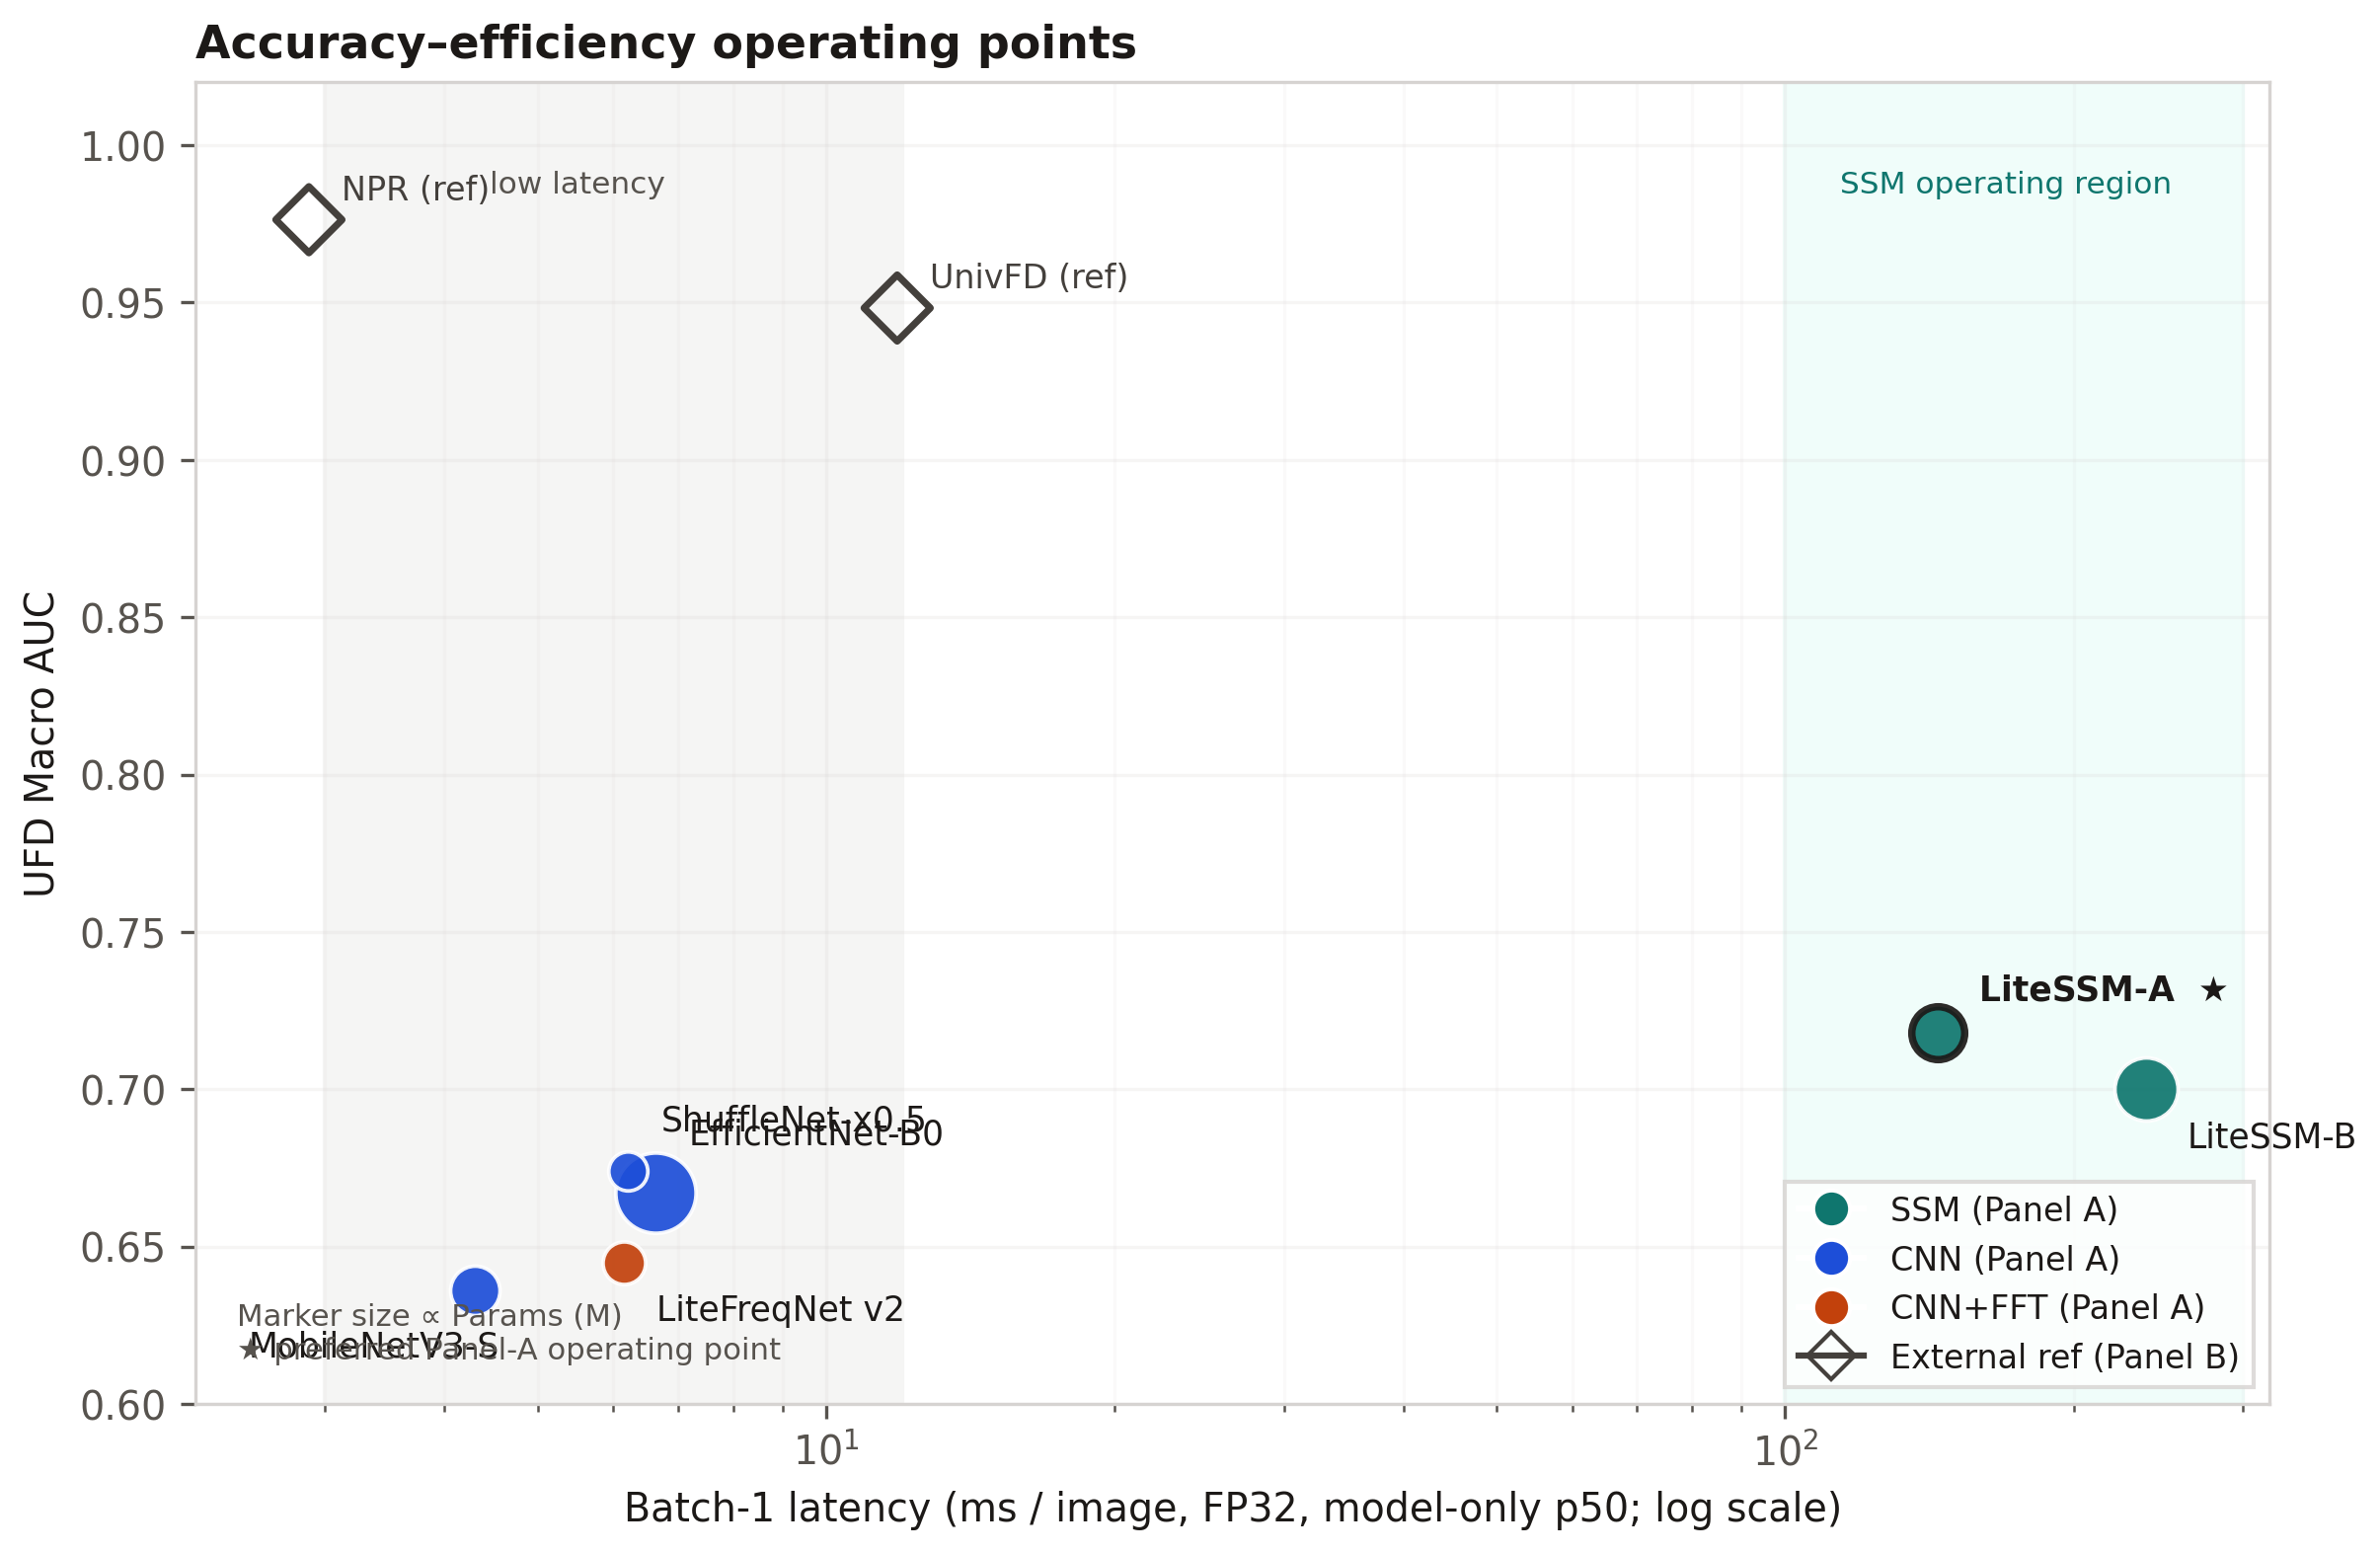
\includegraphics[width=0.92\textwidth]{figures/fig2_pareto_ufd_macro.png}
\caption{Accuracy--efficiency plot using UFD Macro AUC versus batch-1 latency (ms/image, FP32, model-only p50; log $x$-axis).
Filled markers: Panel~A; hollow diamonds: Panel~B references; marker size scales with Params.
The main panel keeps the full $[0.60,1.00]$ Macro range so Panel~B absolute gaps remain visible; the inset magnifies the Panel~A band $[0.60,0.80]$.
LiteSSM-A is marked as the preferred Panel~A operating point (highest Macro, not lowest latency).\label{fig:pareto}}
\end{figure}

\begin{table}[H]
\caption{Operating metrics at a fixed decision threshold.
For Panel~A, the threshold is fitted on the validation set by Youden's $J$ and applied unchanged to ID test and UFD (pooled).
For Panel~B references we report a fixed score threshold of $0.5$ (not recipe-matched Youden).
Bal.\ Acc.\ $=$ $(\mathrm{Sens}+\mathrm{Spec})/2$.\label{tab:operate}}
\scriptsize
\setlength{\tabcolsep}{3.2pt}
\begin{tabularx}{\textwidth}{@{}P{2.15cm}l c *{4}{R}@{}}
\toprule
\textbf{Model} & \textbf{Split} & \textbf{Thr} & \textbf{Bal.} & \textbf{F1} & \textbf{Sens.} & \textbf{Spec.} \\
\midrule
LiteSSM-A & ID & 0.43 & 0.863 & 0.870 & 0.920 & 0.805 \\
LiteSSM-A & UFD pooled & 0.43 & 0.676 & 0.604 & 0.494 & 0.859 \\
EfficientNet-B0 & ID & 0.54 & 0.805 & 0.818 & 0.875 & 0.735 \\
EfficientNet-B0 & UFD pooled & 0.54 & 0.617 & 0.534 & 0.440 & 0.793 \\
LiteFreqNet~v2 & ID & 0.94 & 0.823 & 0.829 & 0.860 & 0.785 \\
LiteFreqNet~v2 & UFD pooled & 0.94 & 0.603 & 0.517 & 0.426 & 0.781 \\
NPR (ref) & ID & 0.50 & 0.867 & 0.862 & 0.830 & 0.905 \\
NPR (ref) & UFD pooled & 0.50 & 0.945 & 0.945 & 0.943 & 0.947 \\
UnivFD (ref) & ID & 0.50 & 0.510 & 0.222 & 0.140 & 0.880 \\
UnivFD (ref) & UFD pooled & 0.50 & 0.818 & 0.781 & 0.650 & 0.986 \\
\bottomrule
\end{tabularx}
\end{table}

\subsection{Within-ID Performance by Content Domain}
\label{sec:domain}

Table~\ref{tab:domain} and Figure~\ref{fig:domain} report domain-wise AUCs on the ID test split.
CelebA-HQ AUCs were near saturation for all models (0.992--0.999).
Bedroom AUCs were substantially lower and separated detectors: SSM models reached $\approx$0.81, EfficientNet-B0 0.777, and remaining compact CNNs 0.677--0.713.
Aggregate ID improvements therefore primarily reflect gains on the harder bedroom domain.

\begin{figure}[H]
\centering
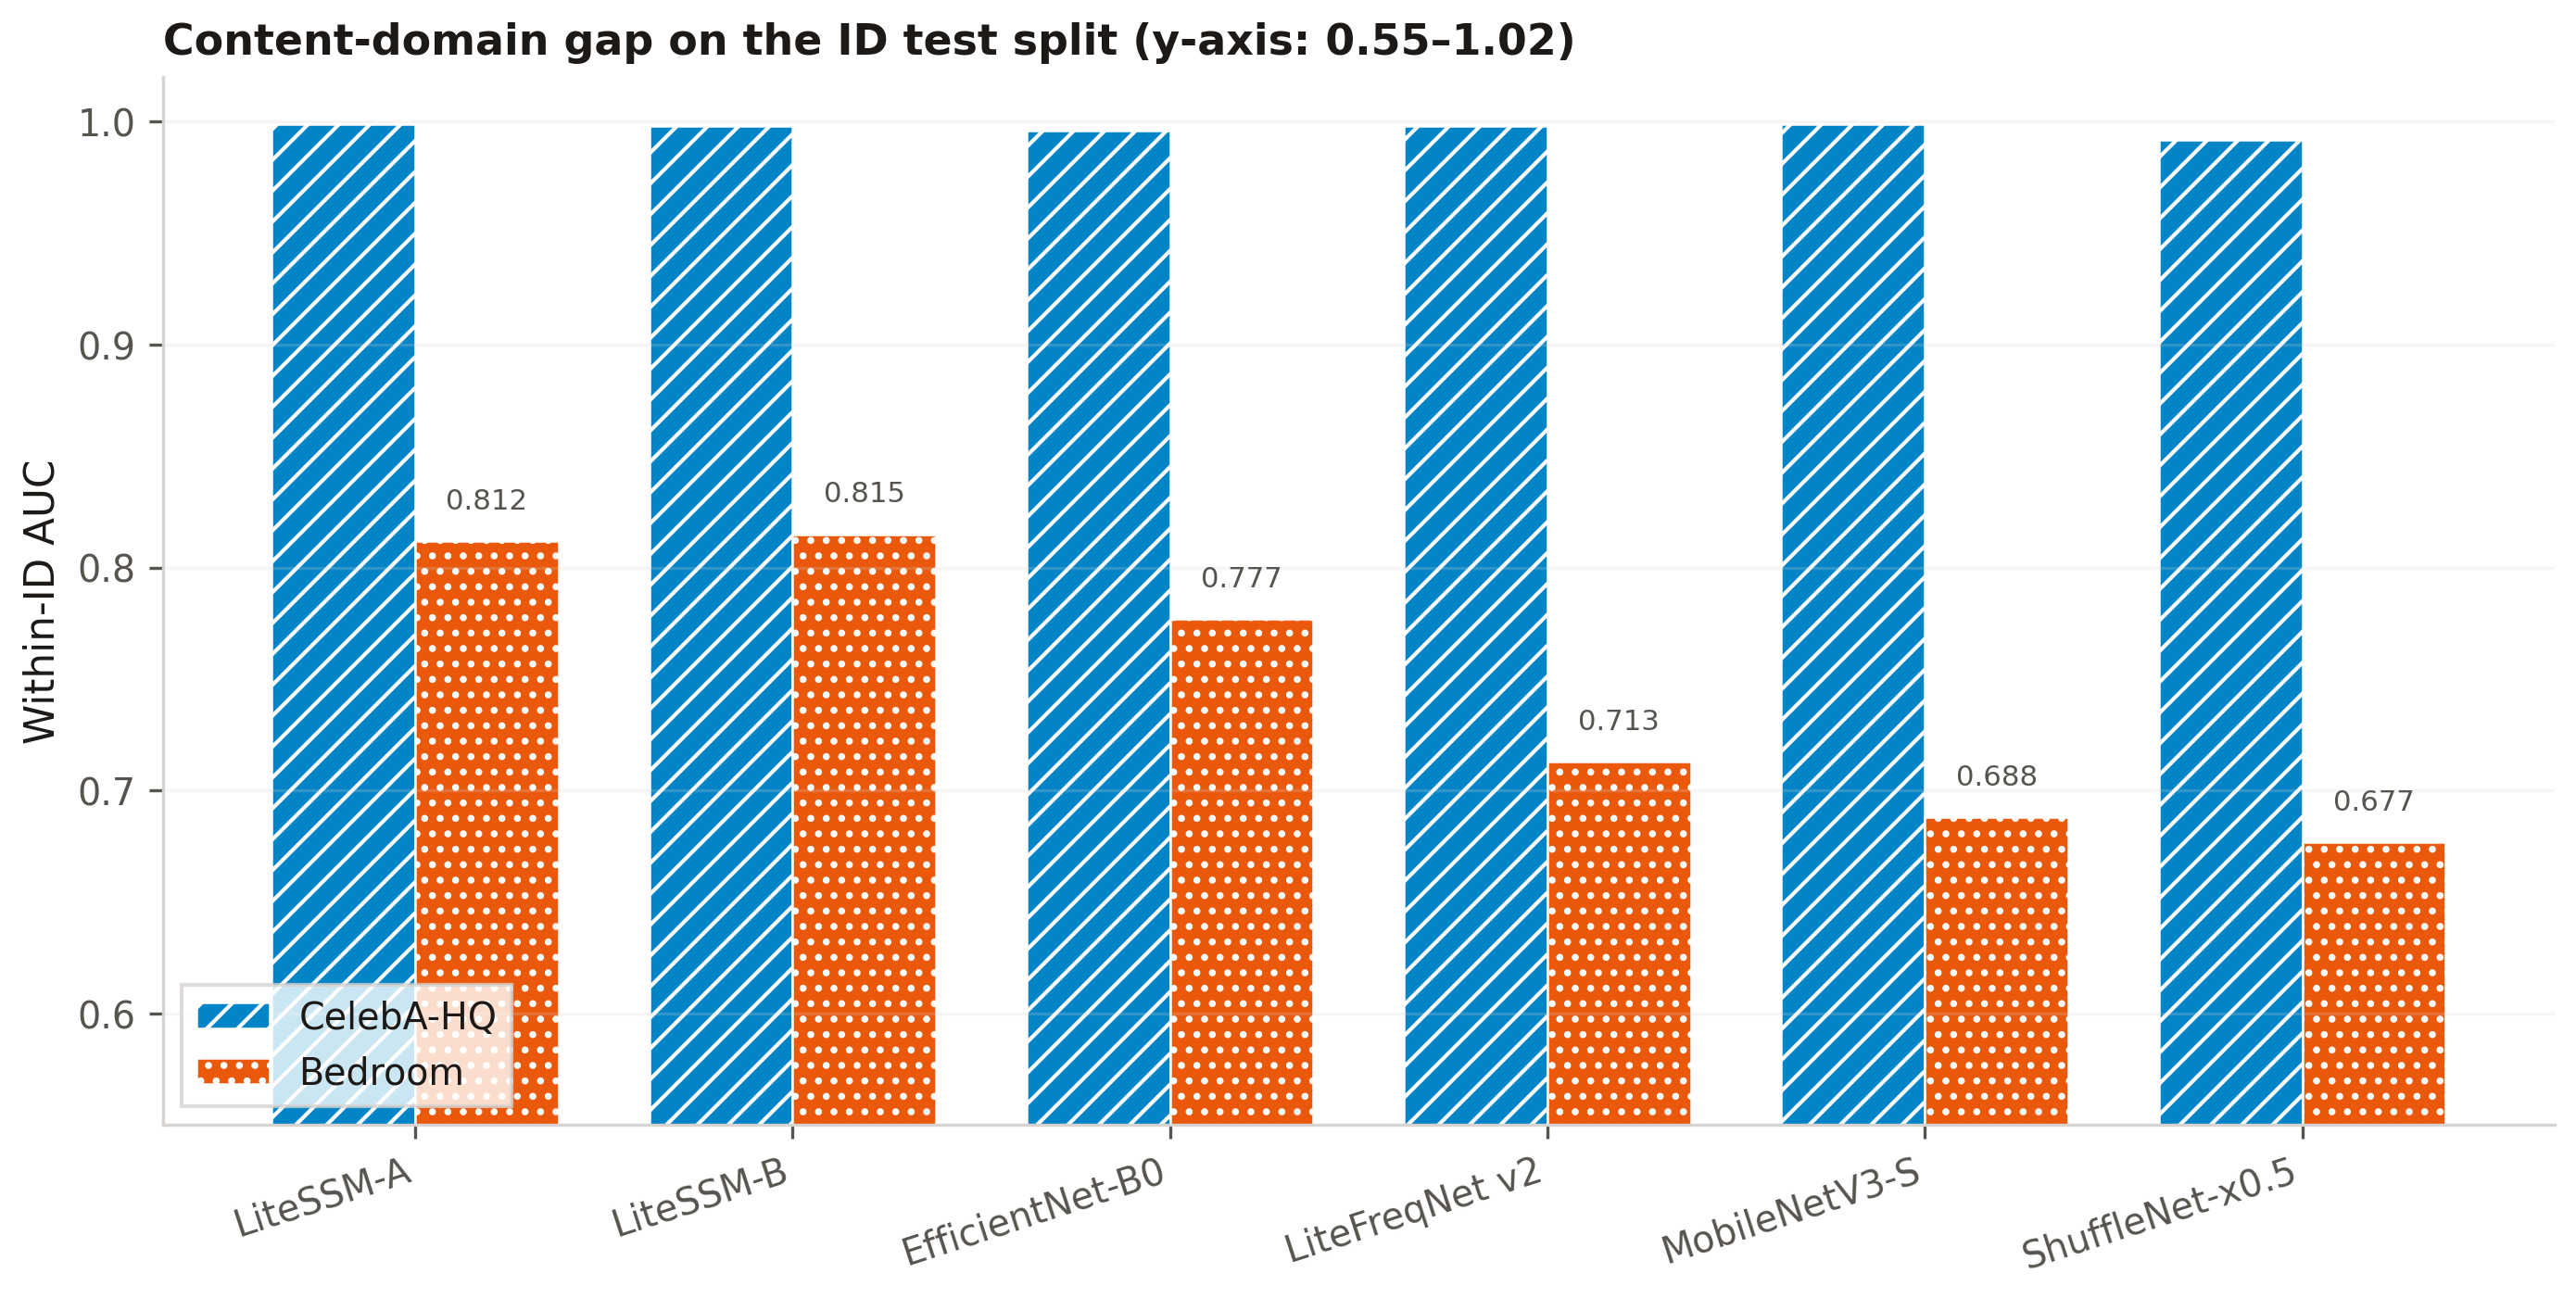
\includegraphics[width=0.95\textwidth]{figures/fig_domain_gap.png}
\caption{Within-ID AUCs by content domain.
CelebA-HQ is near saturation for all Panel~A models; bedroom AUC is the discriminative axis.\label{fig:domain}}
\end{figure}

\begin{table}[H]
\caption{Within-ID AUCs by content domain.\label{tab:domain}}
\scriptsize
\setlength{\tabcolsep}{4pt}
\begin{tabularx}{\textwidth}{@{}P{2.4cm}*{4}{R}@{}}
\toprule
\textbf{Model} & \textbf{ID} & \textbf{CelebA-HQ} & \textbf{Bedroom} & \textbf{Gap} \\
\midrule
LiteSSM-A & 0.946 & 0.999 & 0.812 & 0.187 \\
LiteSSM-B & 0.945 & 0.998 & 0.815 & 0.183 \\
EfficientNet-B0 & 0.929 & 0.996 & 0.777 & 0.219 \\
LiteFreqNet~v2 & 0.906 & 0.998 & 0.713 & 0.285 \\
MobileNetV3-Small & 0.890 & 0.999 & 0.688 & 0.311 \\
ShuffleNetV2-x0.5 & 0.880 & 0.992 & 0.677 & 0.315 \\
\bottomrule
\end{tabularx}
\end{table}

\subsection{Per-Generator Evaluation on UniversalFakeDetect}
\label{sec:ufd}

Table~\ref{tab:ufd} reports per-subset AUCs on UFD~\cite{ojha2023ufd}.
SSM detectors obtain higher Macro averages than the CNN/frequency suite.
Generator identity dominates architecture: Glide subsets are comparatively easy, LDM subsets are weaker, and rankings change across columns.
\textbf{DALL·E remained close to chance for every Panel~A detector (0.451--0.519)}, including both SSMs; the failure is not specific to LiteFreqNet.
Table~\ref{tab:ufd-ext} places the same frozen UFD subsets next to Panel~B pretrained references: UnivFD and NPR remain strong on DALL·E (0.969 / 0.990) and reach substantially higher Macro AUCs.
This contrast indicates a \emph{protocol/panel gap} rather than absolute undetectability of DALL·E under every training paradigm; Panel~B scores are contextual and are \emph{not} ranked against Panel~A under a shared recipe.
Figure~\ref{fig:heatmap} visualizes the Panel~A UFD generator--model matrix.

\begin{table}[H]
\caption{Per-generator AUCs on UFD (400 real + 400 fake per subset).
Macro $=$ equal-weight mean; Min $=$ worst-subset AUC.
Abbreviations: G10/G27/G50 $=$ Glide$_{100,10}$ / Glide$_{100,27}$ / Glide$_{50,27}$; L100/L200/Lcfg $=$ LDM$_{100}$ / LDM$_{200}$ / LDM$_{200,\mathrm{cfg}}$.\label{tab:ufd}}
\scriptsize
\setlength{\tabcolsep}{2.6pt}
\begin{tabularx}{\textwidth}{@{}P{2.05cm}*{10}{R}@{}}
\toprule
\textbf{Model} & \textbf{DALL·E} & \textbf{G10} & \textbf{G27} & \textbf{G50} & \textbf{Guid.} & \textbf{L100} & \textbf{L200} & \textbf{Lcfg} & \textbf{Macro} & \textbf{Min} \\
\midrule
LiteSSM-A & 0.504 & 0.878 & 0.855 & 0.889 & 0.766 & 0.656 & 0.634 & 0.565 & 0.718 & 0.504 \\
LiteSSM-B & 0.483 & 0.859 & 0.831 & 0.868 & 0.788 & 0.622 & 0.611 & 0.535 & 0.700 & 0.483 \\
EfficientNet-B0 & 0.519 & 0.773 & 0.782 & 0.795 & 0.720 & 0.613 & 0.577 & 0.557 & 0.667 & 0.519 \\
LiteFreqNet~v2 & 0.451 & 0.786 & 0.763 & 0.808 & 0.678 & 0.594 & 0.551 & 0.531 & 0.645 & 0.451 \\
MobileNetV3-S & 0.455 & 0.746 & 0.739 & 0.770 & 0.656 & 0.621 & 0.580 & 0.518 & 0.636 & 0.455 \\
ShuffleNet-x0.5 & 0.467 & 0.805 & 0.802 & 0.835 & 0.755 & 0.617 & 0.570 & 0.537 & 0.674 & 0.467 \\
\bottomrule
\end{tabularx}
\end{table}

\begin{table}[H]
\caption{External reference (Panel~B) per-generator AUCs on the same frozen UFD subsets.
Scores are inference-only with public checkpoints and native preprocessing; they contextualize the remaining gap to large-scale pretrained detectors and are not protocol-matched competitors.
Abbreviations follow Table~\ref{tab:ufd}.\label{tab:ufd-ext}}
\scriptsize
\setlength{\tabcolsep}{2.8pt}
\begin{tabularx}{\textwidth}{@{}P{1.7cm}*{9}{R}@{}}
\toprule
\textbf{Detector} & \textbf{DALL·E} & \textbf{G10} & \textbf{G27} & \textbf{G50} & \textbf{Guid.} & \textbf{L100} & \textbf{L200} & \textbf{Lcfg} & \textbf{Macro} \\
\midrule
UnivFD~\cite{ojha2023ufd} & 0.969 & 0.942 & 0.956 & 0.962 & 0.861 & 0.989 & 0.992 & 0.916 & 0.948 \\
NPR~\cite{tan2024npr} & 0.990 & 0.995 & 0.995 & 0.996 & 0.837 & 0.999 & 0.998 & 0.999 & 0.976 \\
\bottomrule
\end{tabularx}
\end{table}

\begin{figure}[H]
\centering
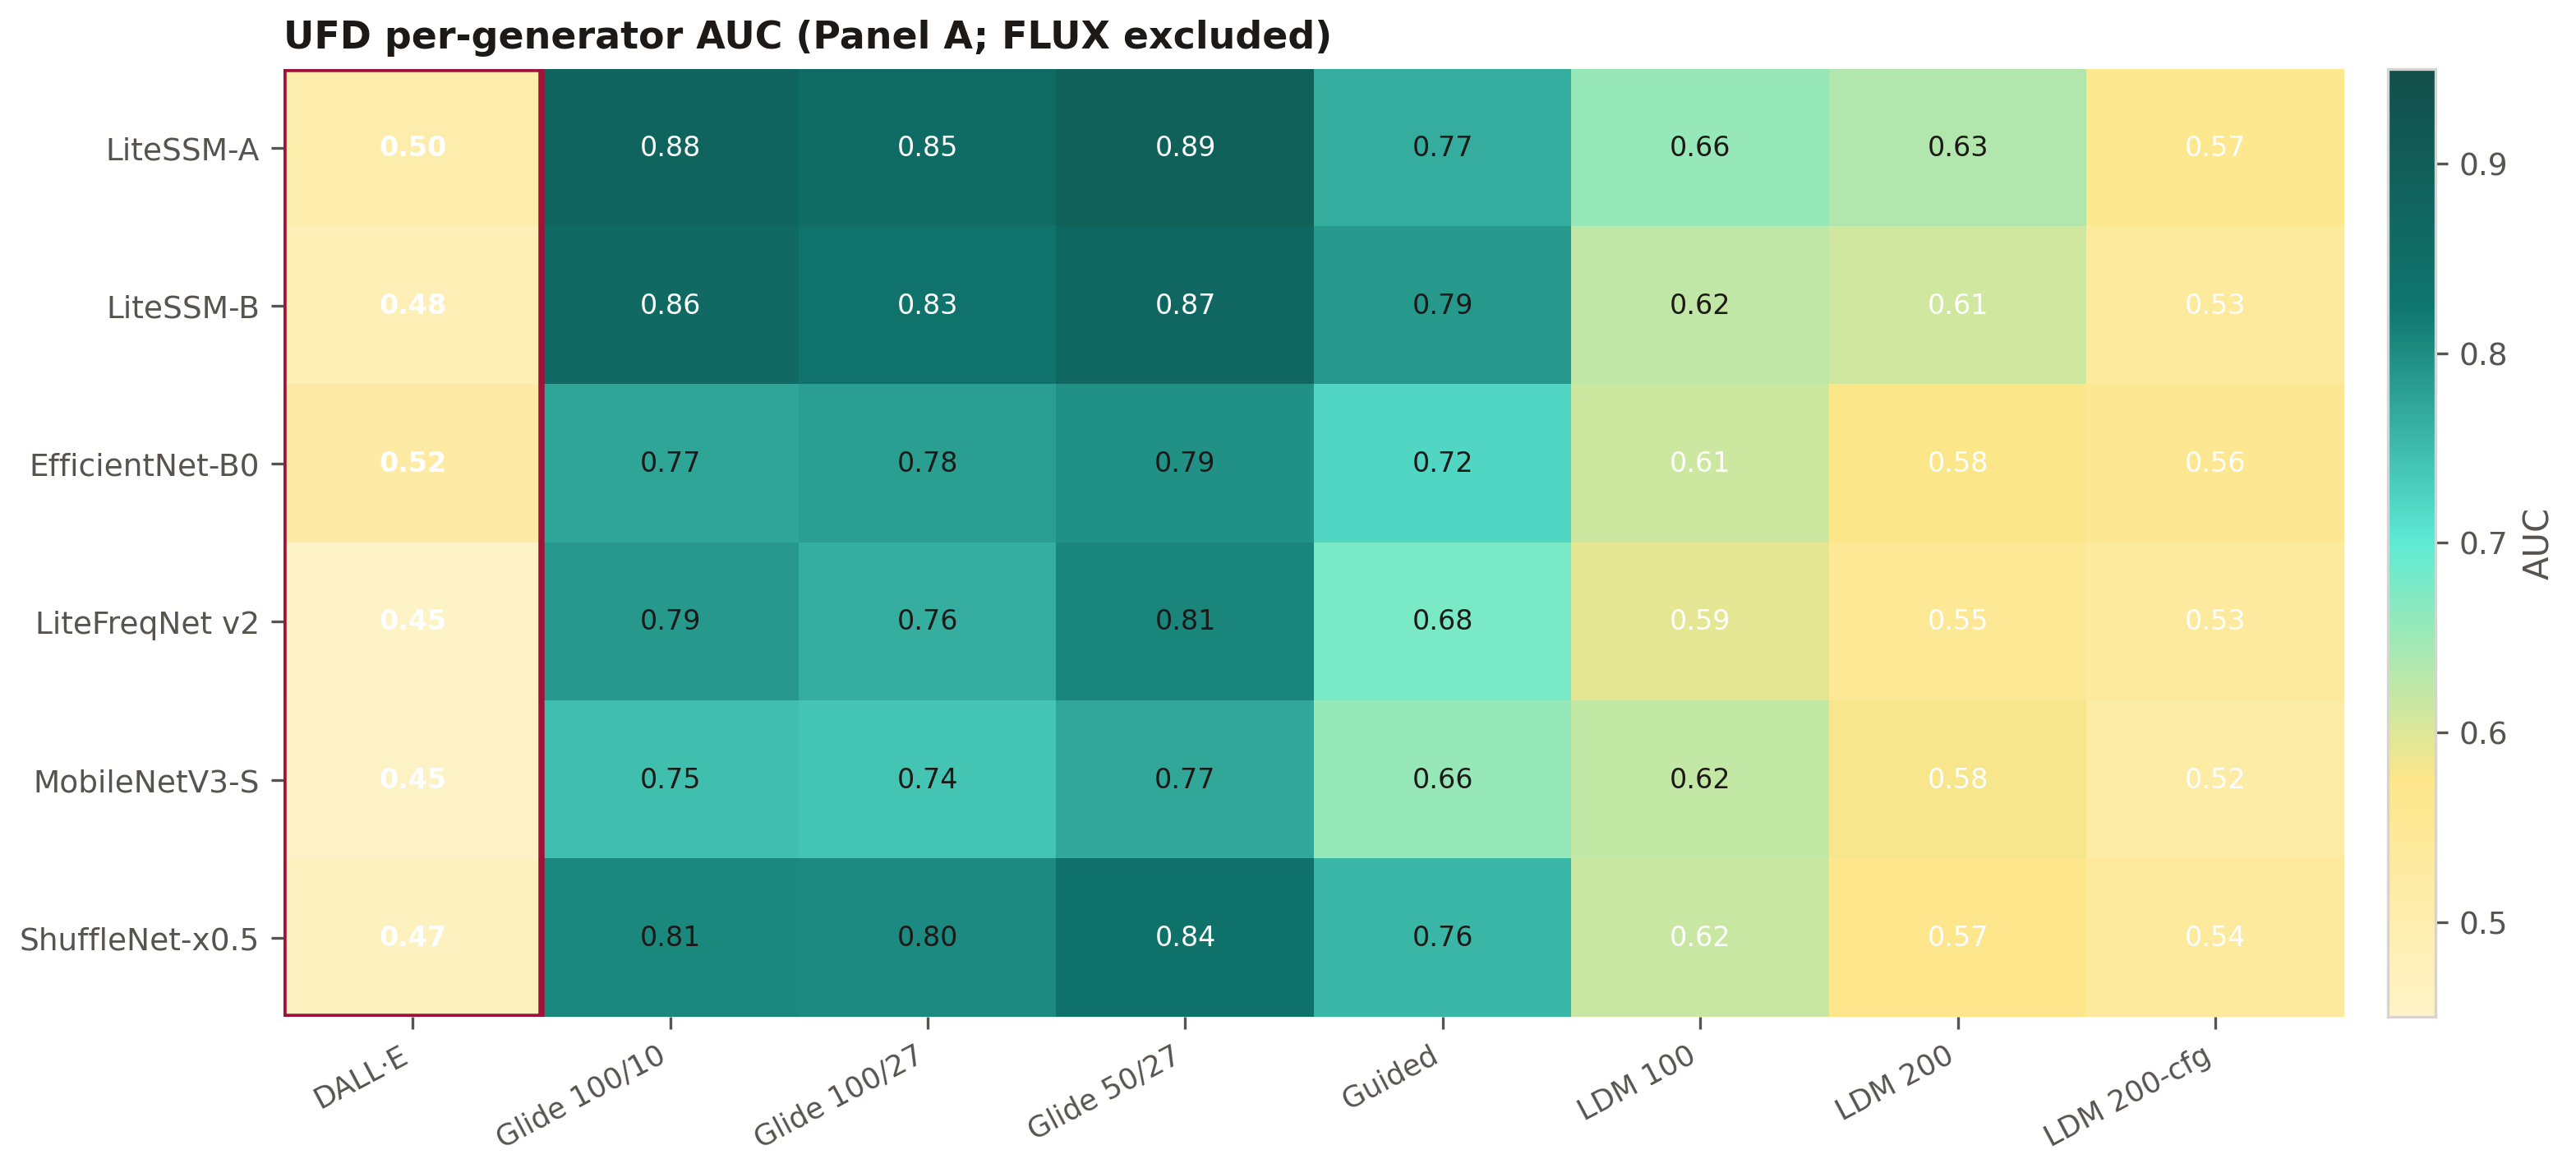
\includegraphics[width=0.98\textwidth]{figures/fig3_generator_heatmap.png}
\caption{Generator--model AUC heatmap for UFD subsets (Panel~A).
The outlined DALL·E column remains near chance for every training-matched compact model.\label{fig:heatmap}}
\end{figure}

Figure~\ref{fig:dalle-diag} diagnoses the DALL·E failure at the score level.
On Glide$_{100,10}$, Panel~A fake/real score mass separates; on DALL·E the two classes largely overlap for LiteSSM-A and EfficientNet-B0, whereas NPR retains clear separation.
A full causal diagnosis would require matched acquisition metadata and spectral decomposition; the present evidence establishes a protocol-level boundary rather than a mechanistic explanation.

\begin{figure}[H]
\centering
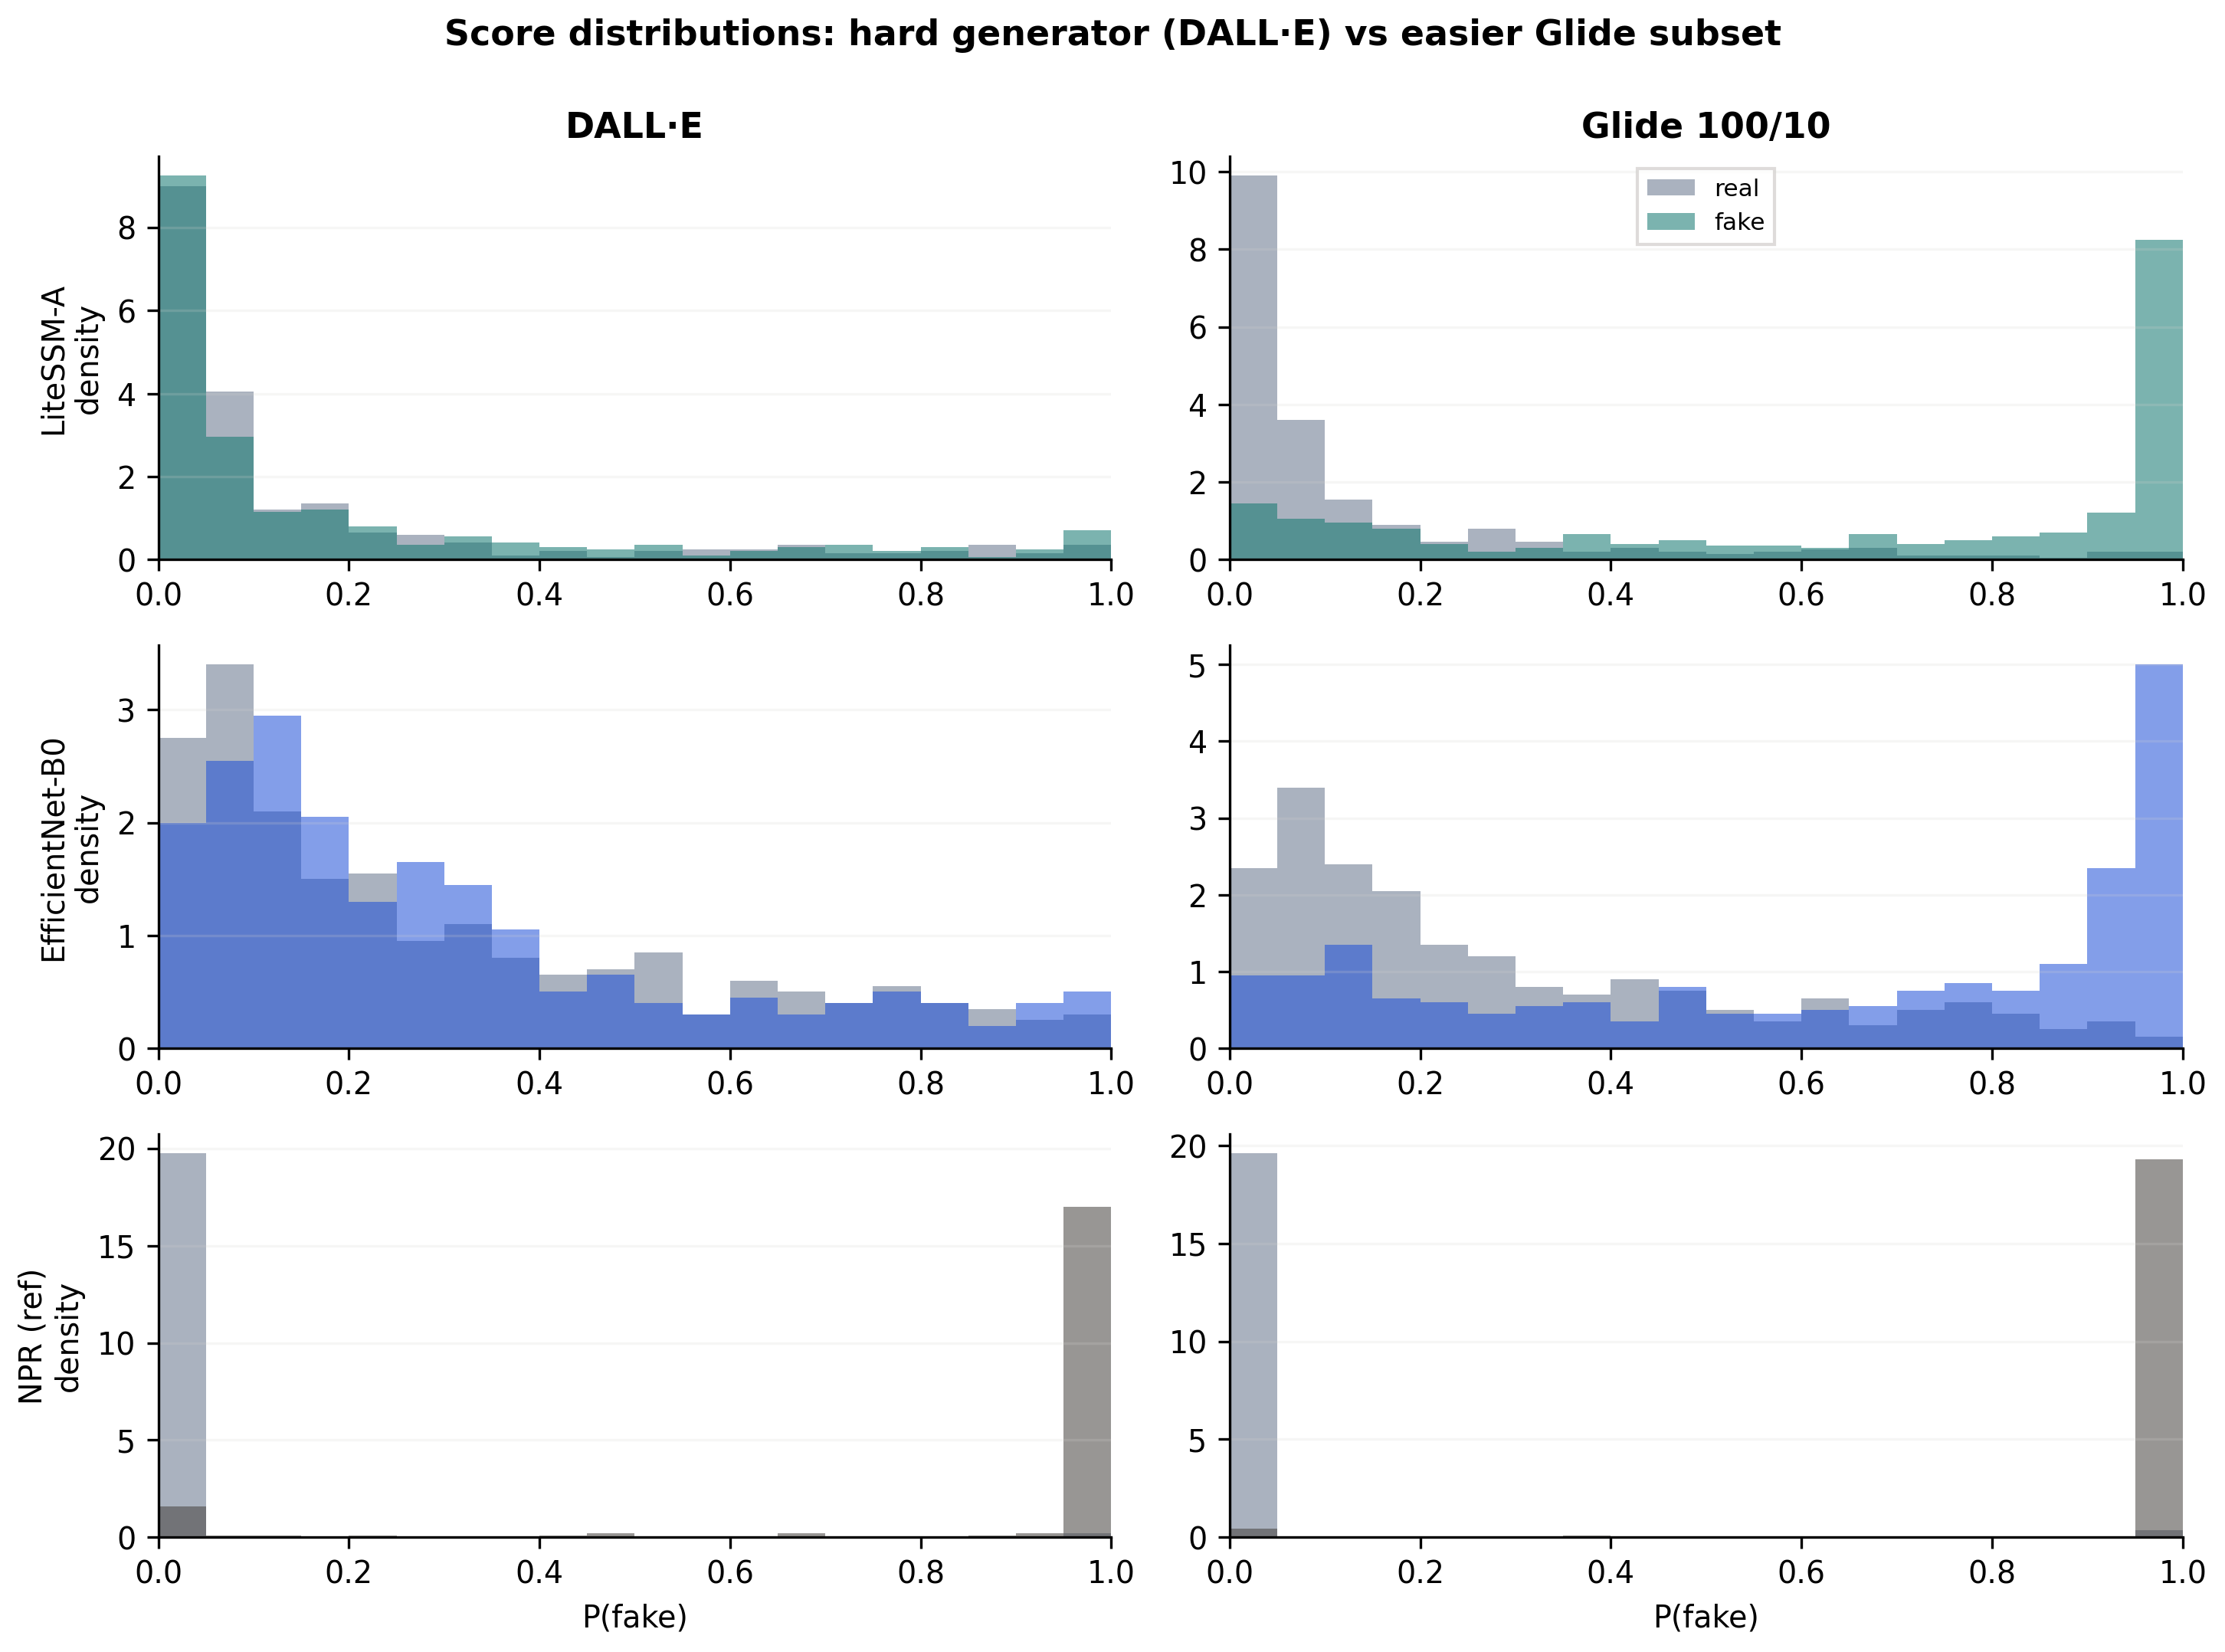
\includegraphics[width=0.98\textwidth]{figures/fig_dalle_score_diag.png}
\caption{Score distributions on UFD DALL·E versus Glide$_{100,10}$ for LiteSSM-A, EfficientNet-B0, and NPR (ref).
Panel~A overlap on DALL·E explains near-chance AUCs; NPR remains separated under a different training paradigm.\label{fig:dalle-diag}}
\end{figure}

\subsection{Robustness under JPEG Q70 Recompression}
\label{sec:jpeg}

Table~\ref{tab:jpeg} compares clean ID AUC with JPEG $Q=70$.
Absolute AUC changes were at most \textbf{0.003} for all models.
Figure~\ref{fig:jpeg-forest} plots paired-bootstrap $\Delta$AUC with 95\% CIs; all intervals include or hug zero, and LiteFreqNet~v2 shows no unique robustness advantage.
The shared observation is stability under the evaluated JPEG Q70 setting, not frequency-module superiority.
A multi-quality absolute-AUC sweep ($Q\in\{95,85,70\}$) remains in Appendix~\ref{app:jpeg}.

\begin{figure}[H]
\centering
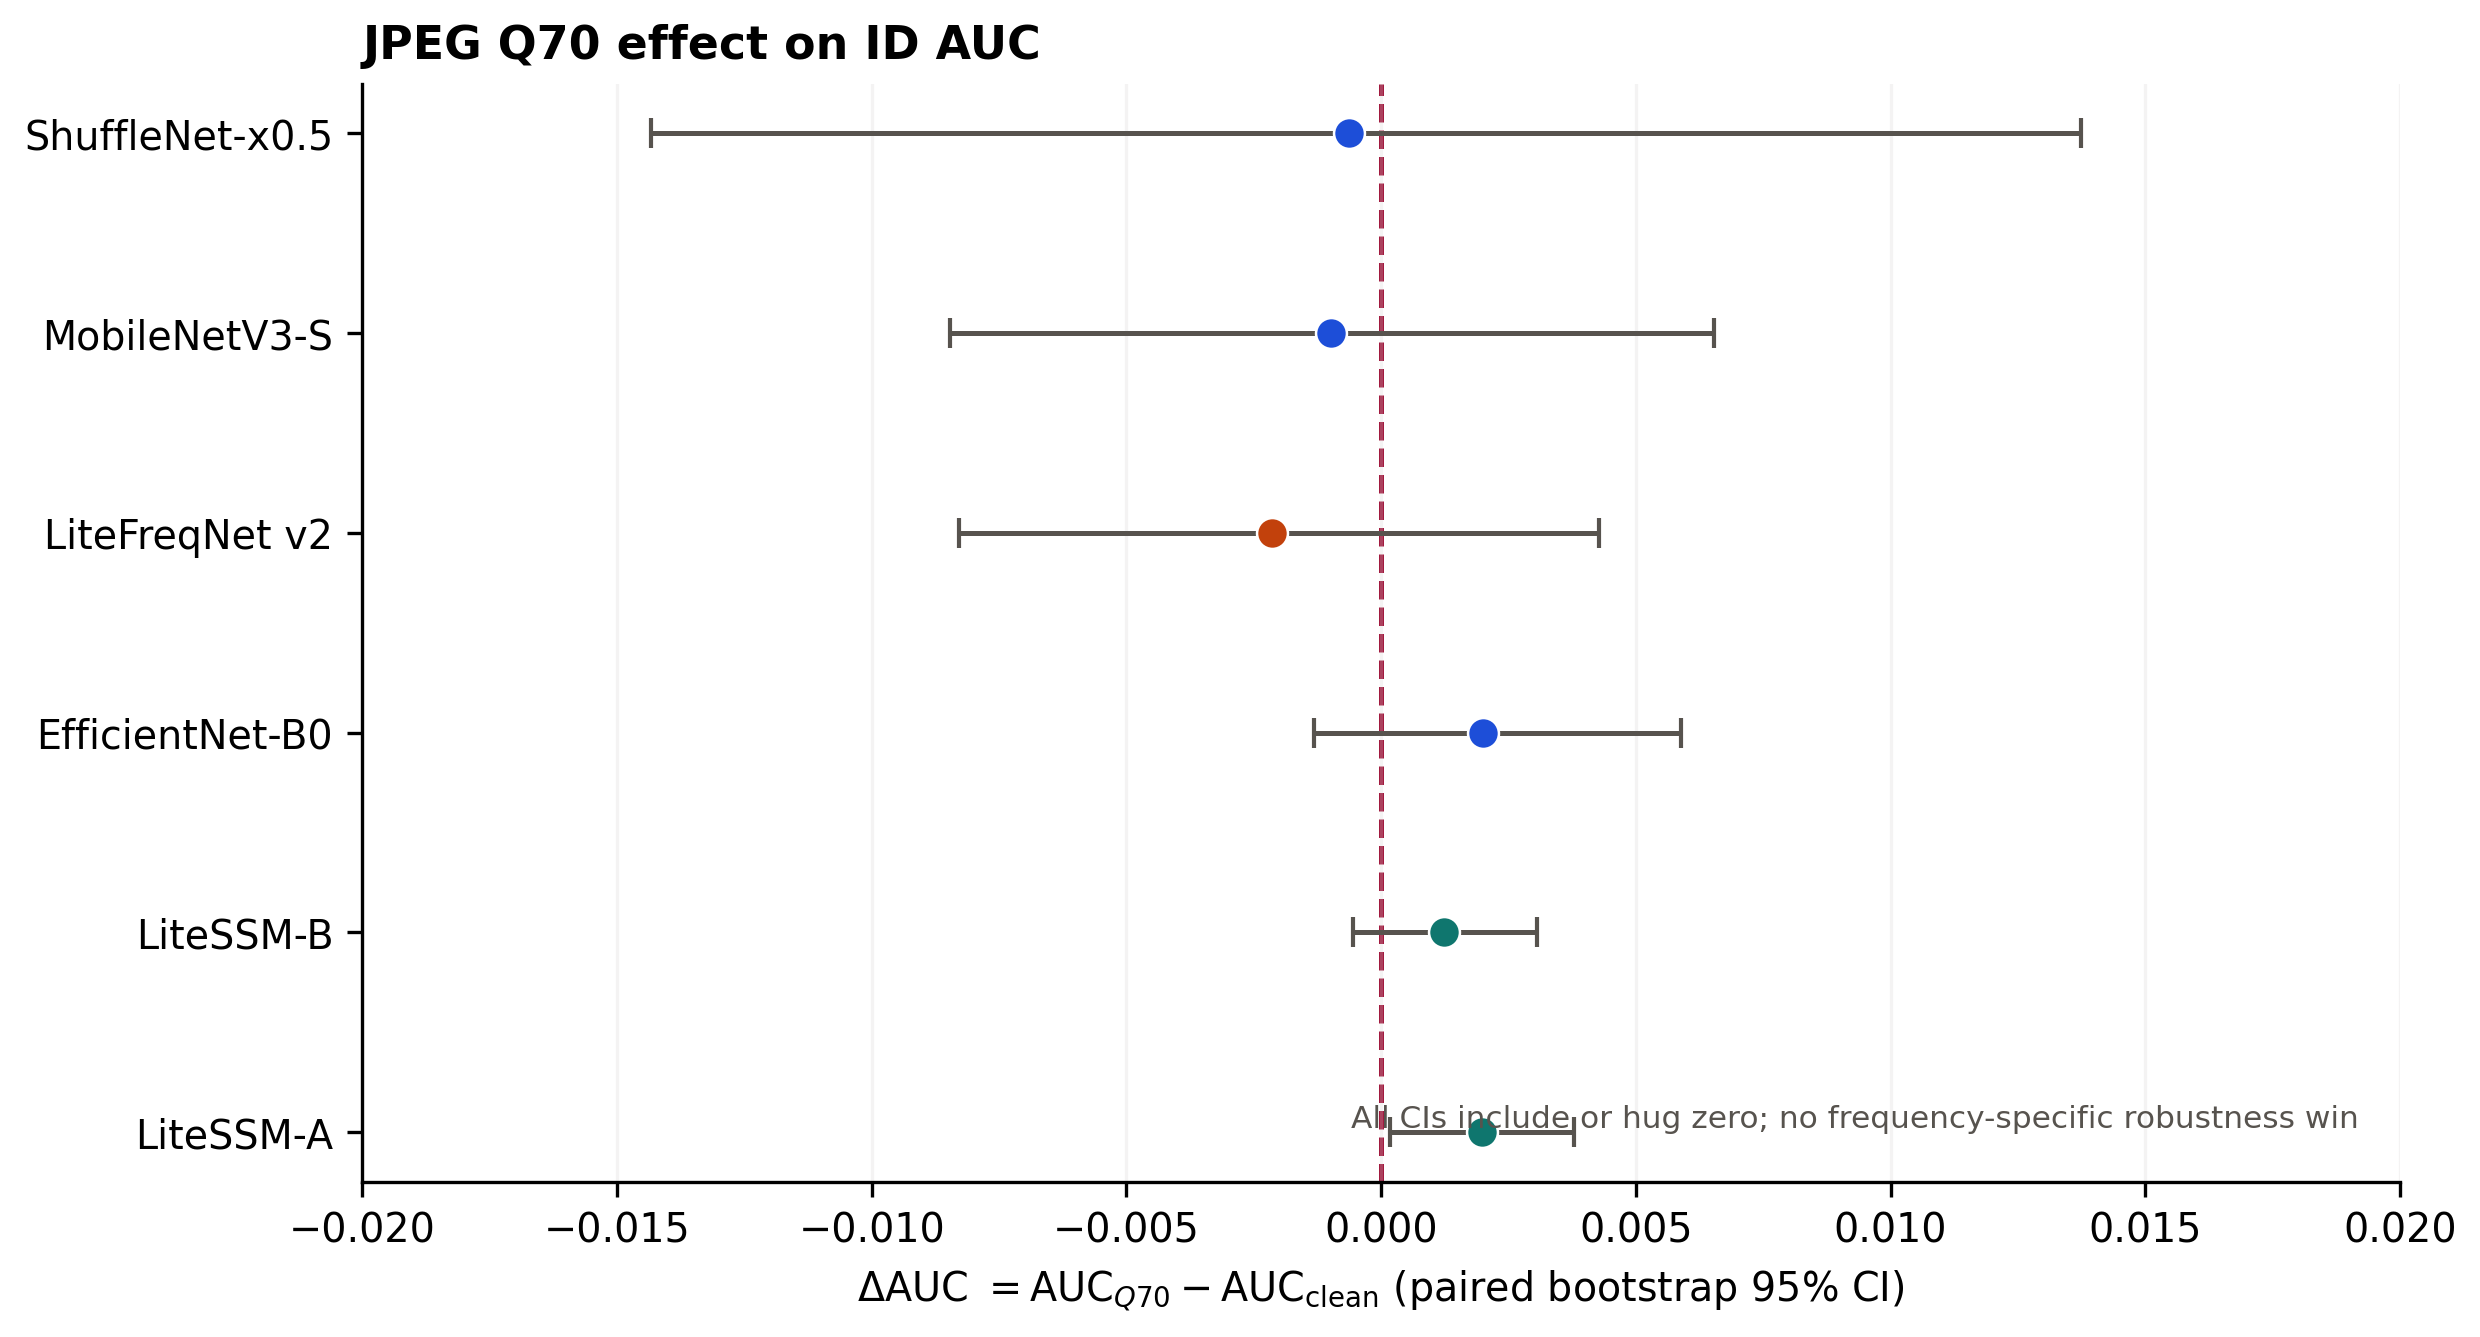
\includegraphics[width=0.92\textwidth]{figures/fig_jpeg_delta_forest.png}
\caption{Forest plot of ID $\Delta$AUC $=\mathrm{AUC}_{Q70}-\mathrm{AUC}_{\mathrm{clean}}$ with paired bootstrap 95\% CIs ($B=1000$, seed~42).
The dashed line marks zero effect.\label{fig:jpeg-forest}}
\end{figure}

\begin{table}[H]
\caption{ID AUC under JPEG Q70 recompression.\label{tab:jpeg}}
\scriptsize
\setlength{\tabcolsep}{4pt}
\begin{tabularx}{\textwidth}{@{}P{2.4cm}*{4}{R}@{}}
\toprule
\textbf{Model} & \textbf{Clean} & \textbf{Q70} & \textbf{$\Delta$AUC} & \textbf{$\Delta$CI95} \\
\midrule
LiteSSM-A & 0.946 & 0.948 & $+0.002$ & $[+0.000,\ +0.004]$ \\
LiteSSM-B & 0.945 & 0.946 & $+0.001$ & $[-0.001,\ +0.003]$ \\
EfficientNet-B0 & 0.929 & 0.931 & $+0.002$ & $[-0.001,\ +0.006]$ \\
LiteFreqNet~v2 & 0.906 & 0.904 & $-0.002$ & $[-0.008,\ +0.004]$ \\
MobileNetV3-Small & 0.890 & 0.889 & $-0.001$ & $[-0.009,\ +0.007]$ \\
ShuffleNetV2-x0.5 & 0.880 & 0.879 & $-0.001$ & $[-0.014,\ +0.014]$ \\
\bottomrule
\end{tabularx}
\end{table}

\subsection{Ablation and Frequency-Module Transferability}

Replacing early concatenation with gated residual fusion recovered usable thresholds after a probability-collapse failure in the initial LiteFreq design; LiteFreqNet~v2 is retained in the main tables.
Table~\ref{tab:freq-abl} summarizes frequency-branch ablations under the bake-off protocol.
Attaching the frequency branch to SSM backbones slightly reduced ID and OOD Pooled AUC; removing the frequency branch from LiteFreqNet likewise hurts ID/OOD Pooled.
Frequency-branch variants for SSM backbones (and the LiteFreq no-frequency control) were evaluated with OOD Pooled AUC; \textbf{UFD Macro was not recomputed for these ablations}.
Frequency injection was therefore not a transferable free upgrade across architectures in this protocol.

\begin{table}[H]
\caption{Frequency-module ablation under the locked bake-off protocol.
UFD Macro is reported only for primary main-table checkpoints; ablation rows use ID and OOD Pooled only.\label{tab:freq-abl}}
\scriptsize
\setlength{\tabcolsep}{4pt}
\begin{tabularx}{\textwidth}{@{}P{3.2cm}*{3}{R}@{}}
\toprule
\textbf{Model} & \textbf{ID} & \textbf{OOD Pooled} & \textbf{UFD Macro} \\
\midrule
LiteSSM-A & 0.946 & 0.712 & 0.718 \\
LiteSSM-A + freq & 0.937 & 0.696 & -- \\
LiteSSM-B & 0.945 & 0.722 & 0.700 \\
LiteSSM-B + freq & 0.938 & 0.695 & -- \\
LiteFreqNet~v2 & 0.906 & 0.698 & 0.645 \\
LiteFreqNet (no-freq) & 0.857 & 0.648 & -- \\
\bottomrule
\end{tabularx}
\end{table}

An exploratory FLUX evaluation was additionally conducted; however, because the real and synthetic subsets were not content- and acquisition-matched, the results are reported only as supplementary evidence in Appendix~\ref{app:flux} and are \emph{not} used to support architecture-level conclusions.


%%%%%%%%%%%%%%%%%%%%%%%%%%%%%%%%%%%%%%%%%%
\section{Discussion}
\label{sec:discussion}
\subsection{Why UFD Macro and OOD Pooled Rankings Differ}

LiteSSM-B obtains a higher \textbf{OOD Pooled} AUC (\textbf{0.722}) than LiteSSM-A (\textbf{0.712}), yet a lower \textbf{UFD Macro} (\textbf{0.700} vs.\ \textbf{0.718}).
Pooled AUC weights every OOD sample equally and can amplify easier or larger subsets inside \texttt{test\_ood.jsonl}.
Macro AUC averages generator-level AUCs with equal weight and remains sensitive to consistently weak generators such as DALL·E.
We therefore treat \textbf{UFD Macro as the primary cross-generator summary} for deployment-oriented reporting and keep pooled OOD as a secondary aggregate that must not substitute for Macro in the text or tables.

\subsection{SSM as a Stronger Deployment Point---Not a Universal Detector}

Across ID, UFD Macro, and bedroom-domain ID, LiteSSM-A occupies a favorable accuracy--size region under the evaluated latency budget.
LiteSSM-B is close on ID and competitive on several OOD views, but is heavier and slower; the LiteSSM-A--LiteSSM-B ID gap is CI-overlapping.
These gains do \emph{not} imply a universal or generator-agnostic detector: worst-generator AUC remains near chance for both SSMs.
The appropriate claim is narrower---under a matched lightweight protocol, SSM backbones improved average transfer relative to compact CNN baselines, while generator-specific collapse persisted.
LiteSSM-A is preferred for its highest Panel~A UFD Macro together with a locked batch-32 throughput of 226 images/s, not because it minimizes absolute batch-1 latency.

\subsection{Boundaries Exposed by Bedroom Content and DALL·E}

Near-ceiling CelebA-HQ AUCs show that aggregate ID scores can look strong even when a substantial content domain remains difficult (Section~\ref{sec:domain}).
Bedroom performance ($\approx$0.68--0.81) is where models separate and where SSM gains are most visible.
DALL·E exposes an orthogonal \textbf{generator} boundary: chance-level AUCs across CNN and SSM alike indicate that the limitation is not an artifact of LiteFreqNet alone (Section~\ref{sec:ufd}).

\subsection{Frequency Enhancement Is Not Universally Helpful}

LiteFreqNet~v2 did not win ID, UFD Macro, bedroom, or JPEG uniqueness.
Attaching a similar frequency branch to SSM backbones slightly hurt bake-off ID/OOD Pooled metrics.
Under the evaluated JPEG Q70 recompression setting, all compact models moved by at most 0.003 AUC (Section~\ref{sec:jpeg}); stability was shared rather than frequency-specific.
We therefore interpret frequency features as protocol- and architecture-dependent, not as a general recipe for lightweight AIGC detection.

\subsection{Limitations}

Training used a fixed no-pretraining recipe, a single training seed, and two DF training sources.
Bootstrap intervals quantify test-sample uncertainty but do not capture training stochasticity.
UFD Macro depends on the chosen subset list and per-class caps.
JPEG analysis focuses on Q70 for the main claim.
External reference detectors (UnivFD, NPR) use publicly released pretrained weights and native preprocessing; they contextualize performance and are not training-matched competitors.
An unmatched FLUX subset is reported only in Appendix~\ref{app:flux}~\cite{flux2024}.
Reported SSMs are study-specific pure-PyTorch classifiers for controlled comparison, not official architecture releases or vendor-kernel peaks.
Deepfake video and legal-forensics claims are out of scope.

\subsection{Practical Takeaway}

For practitioners selecting one compact still-image detector from the training-matched suite, \textbf{LiteSSM-A} is the recommended operating point under the evaluated latency budget, paired with explicit monitoring for difficult generators (e.g., DALL·E-like sources) and content domains (e.g., indoor scenes), rather than an assumption of uniform reliability.


%%%%%%%%%%%%%%%%%%%%%%%%%%%%%%%%%%%%%%%%%%
\section{Conclusions}
\label{sec:conclusions}
We conducted a reproducible, protocol-matched comparison of compact CNN, frequency-aware, and state-space detectors for AI-generated still-image detection under a locked no-pretraining recipe.
Using frozen splits and clearly separated metrics---especially \textbf{UFD Macro} versus \textbf{OOD Pooled}---we find that \textbf{LiteSSM-A} offers the most favorable generalization--efficiency operating point among Panel~A models, combining strong ID performance, the highest UFD Macro AUC in that panel, and improved bedroom-domain behavior at moderate model size, with a locked batch-32 throughput of 226 images/s.
It is selected for that trade-off rather than for lowest absolute batch-1 latency.
LiteSSM-B remains a competitive SSM alternative under some aggregates (including a higher OOD Pooled AUC of 0.722).

Equally important are the boundaries that remain: DALL·E detection stays near chance for all Panel~A architectures while Panel~B pretrained references remain strong on the same subset; CelebA-HQ saturation masks bedroom difficulty in pooled ID scores; JPEG Q70 leaves all evaluated compact models nearly unchanged without crowning a frequency-specific winner; and frequency branches do not universally improve SSM or CNN transfer.
Relative to LAID and LOTA~\cite{chivaran2025laid,wang2025lota}, the reusable knowledge is the controlled evidence organization---generator-macro OOD, domain decomposition, worst-generator failure, and measured latency/throughput under one disclosed protocol---not a claim of a new universal lightweight detector.
These results support selecting LiteSSM-A as a practical compact operating point while rejecting narratives of universal, domain-invariant, or broadly compression-robust detection beyond the evaluated settings.

Future work will pre-register a modern-generator augmentation protocol with an independent development split, targeting improved FLUX/SDXL transfer without degrading the frozen UFD Macro baseline, and without treating held-out modern-generator gains as method-selection evidence.
Additional directions include extending multi-seed reporting beyond the LiteSSM-A / EfficientNet-B0 appendix probe and hardening worst-generator monitoring while preserving the compact, fully disclosed protocol used here.


%%%%%%%%%%%%%%%%%%%%%%%%%%%%%%%%%%%%%%%%%%
\appendix
\section{Exploratory Evaluation on the Unmatched FLUX Subset}
\label{app:flux}

An exploratory FLUX evaluation was conducted independently of the locked training protocol.
We generated 100 images with FLUX.1-\texttt{schnell}~\cite{flux2024} (Diffusers \texttt{FluxPipeline}, \texttt{bfloat16}, CPU offload, 4 steps, guidance 0.0, \texttt{max\_sequence\_length}=256, seeds $42+i$, ten cycled English prompts) and paired them with 100 DiffusionForensics real images (seed~42).
Because the real and synthetic subsets were \textbf{not} content- and acquisition-matched---native resolutions differ, PNG vs.\ JPEG containers differ, and residual pipeline cues cannot be ruled out---these results are reported only as supplementary evidence and are \textbf{not} used to support architecture-level conclusions in the main text.

Table~\ref{tab:flux-app} lists AUCs with bootstrap 95\% CIs ($B=1000$, seed~42).
The LiteSSM-A vs.\ LiteSSM-B difference CI includes zero ($\Delta$AUC $+0.026$ $[-0.006,\ 0.057]$).

\begin{table}[H]
\caption{Exploratory evaluation on the unmatched FLUX subset ($n=200$).\label{tab:flux-app}}
\scriptsize
\setlength{\tabcolsep}{4pt}
\begin{tabularx}{\textwidth}{@{}P{2.4cm}l*{2}{R}@{}}
\toprule
\textbf{Model} & \textbf{Arch} & \textbf{AUC} & \textbf{95\% CI} \\
\midrule
LiteSSM-A & SSM & 0.782 & $[0.719,\ 0.841]$ \\
LiteSSM-B & SSM & 0.757 & $[0.688,\ 0.819]$ \\
MobileNetV3-Small & CNN & 0.685 & $[0.606,\ 0.758]$ \\
LiteFreqNet~v2 & CNN+FFT & 0.677 & $[0.601,\ 0.749]$ \\
EfficientNet-B0 & CNN & 0.657 & $[0.579,\ 0.728]$ \\
\bottomrule
\end{tabularx}
\end{table}


%%%%%%%%%%%%%%%%%%%%%%%%%%%%%%%%%%%%%%%%%%
\vspace{6pt}

\authorcontributions{Conceptualization, methodology, software, validation, formal analysis, investigation, resources, data curation, writing---original draft preparation, writing---review and editing, visualization, and project administration, K.C. The author has read and agreed to the published version of the manuscript.}

\funding{This research received no external funding.}

\institutionalreview{Not applicable.}

\informedconsent{Not applicable.}

\dataavailability{Original images come from public datasets (DiffusionForensics; UniversalFakeDetect) and must be obtained from their providers under the original licenses; we do not redistribute raw third-party images. Frozen manifests (sample IDs and paths), SHA256 digests, prediction/efficiency summaries, and table-regeneration scripts are available at \url{https://github.com/opencodingscau/lite-aigc-detect} (release \texttt{v1.0.0-paper.2}) and archived at Zenodo with version DOI \url{https://doi.org/10.5281/zenodo.21604045} (concept DOI \url{https://doi.org/10.5281/zenodo.21604044}). Panel~A self-trained checkpoints follow \texttt{checkpoints/README.md} and are redistributed only when training-data licenses permit; Panel~B detectors (UnivFD, NPR) must be obtained from their official releases. The unmatched FLUX exploratory subset is documented in Appendix~\ref{app:flux}; redistribution follows the same license constraints as the source real pool and FLUX model terms.}

\acknowledgments{The author thanks the maintainers of the publicly released datasets and reference detectors used in this study.}

\conflictsofinterest{The author declares no conflicts of interest.}

%%%%%%%%%%%%%%%%%%%%%%%%%%%%%%%%%%%%%%%%%%
\abbreviations{Abbreviations}{
The following abbreviations are used in this manuscript:\\

\noindent
\begin{tabular}{@{}ll}
AUC & Area under the ROC curve\\
CNN & Convolutional neural network\\
DF & DiffusionForensics\\
FPS & Frames per second\\
ID & In-distribution\\
OOD & Out-of-distribution\\
SSM & State-space model\\
UFD & UniversalFakeDetect\\
\end{tabular}
}

%%%%%%%%%%%%%%%%%%%%%%%%%%%%%%%%%%%%%%%%%%
\begin{adjustwidth}{-\extralength}{0cm}
\reftitle{References}

% ACS format (Applied Sciences)
\isAPAandChicago{}{%
\begin{thebibliography}{999}

\bibitem[Tan and Le(2019)]{tan2019efficientnet}
Tan, M.; Le, Q.V. EfficientNet: Rethinking model scaling for convolutional neural networks. In Proceedings of the 36th International Conference on Machine Learning (ICML), Long Beach, CA, USA, 9--15 June 2019; Proceedings of Machine Learning Research; Vol.~97, pp.~6105--6114. Available online: \url{https://proceedings.mlr.press/v97/tan19a.html} (accessed on 26 July 2026).

\bibitem[Howard et al.(2019)]{howard2019mobilenetv3}
Howard, A.; Sandler, M.; Chu, G.; Chen, L.C.; Chen, B.; Tan, M.; Wang, W.; Zhu, Y.; Pang, R.; Vasudevan, V.; et al. Searching for MobileNetV3. In Proceedings of the IEEE/CVF International Conference on Computer Vision (ICCV), Seoul, Republic of Korea, 27 October--2 November 2019; pp.~1314--1324. https://doi.org/10.1109/ICCV.2019.00140.

\bibitem[Ma et al.(2018)]{ma2018shufflenet}
Ma, N.; Zhang, X.; Zheng, H.T.; Sun, J. ShuffleNet V2: Practical guidelines for efficient CNN architecture design. In Proceedings of the European Conference on Computer Vision (ECCV), Munich, Germany, 8--14 September 2018; Lecture Notes in Computer Science; Springer: Cham, Switzerland, 2018; Vol.~11218, pp.~122--138. https://doi.org/10.1007/978-3-030-01264-9\_8.

\bibitem[Ojha et al.(2023)]{ojha2023ufd}
Ojha, U.; Li, Y.; Lee, Y.J. Towards universal fake image detectors that generalize across generative models. In Proceedings of the IEEE/CVF Conference on Computer Vision and Pattern Recognition (CVPR), Vancouver, BC, Canada, 18--22 June 2023; pp.~24480--24489. https://doi.org/10.1109/CVPR52729.2023.02345.

\bibitem[Wang et al.(2020)]{wang2020cnn}
Wang, S.Y.; Wang, O.; Zhang, R.; Owens, A.; Efros, A.A. CNN-generated images are surprisingly easy to spot\ldots for now. In Proceedings of the IEEE/CVF Conference on Computer Vision and Pattern Recognition (CVPR), Seattle, WA, USA, 13--19 June 2020; pp.~8695--8704. https://doi.org/10.1109/CVPR42600.2020.00872.

\bibitem[Frank et al.(2020)]{frank2020freq}
Frank, J.; Eisenhofer, T.; Sch{\"o}nherr, L.; Fischer, A.; Kolossa, D.; Holz, T. Leveraging frequency analysis for deep fake image recognition. In Proceedings of the 37th International Conference on Machine Learning (ICML), Virtual Event, 13--18 July 2020; Proceedings of Machine Learning Research; Vol.~119, pp.~3247--3258. Available online: \url{https://proceedings.mlr.press/v119/frank20a.html} (accessed on 26 July 2026).

\bibitem[Gu and Dao(2023)]{gu2023mamba}
Gu, A.; Dao, T. Mamba: Linear-time sequence modeling with selective state spaces. {\em arXiv} {\bf 2023}, arXiv:2312.00752. https://doi.org/10.48550/arXiv.2312.00752.

\bibitem[Tan et al.(2024)]{tan2024npr}
Tan, C.; Zhao, Y.; Wei, S.; Gu, G.; Liu, P.; Wei, Y. Rethinking the up-sampling operations in CNN-based generative network for generalizable deepfake detection. In Proceedings of the IEEE/CVF Conference on Computer Vision and Pattern Recognition (CVPR), Seattle, WA, USA, 16--22 June 2024; pp.~28130--28139. https://doi.org/10.1109/CVPR52733.2024.02657.

\bibitem[Wang et al.(2023)]{wang2023dire}
Wang, Z.; Bao, J.; Zhou, W.; Wang, W.; Hu, H.; Chen, H.; Li, H. DIRE for diffusion-generated image detection. In Proceedings of the IEEE/CVF International Conference on Computer Vision (ICCV), Paris, France, 2--6 October 2023; pp.~22445--22455. https://doi.org/10.1109/ICCV51070.2023.02051.

\bibitem[Corvi et al.(2023)]{corvi2023diffusion}
Corvi, R.; Cozzolino, D.; Zingarini, G.; Poggi, G.; Nagano, K.; Verdoliva, L. On the detection of synthetic images generated by diffusion models. In Proceedings of the IEEE International Conference on Acoustics, Speech and Signal Processing (ICASSP), Rhodes Island, Greece, 4--10 June 2023; pp.~1--5. https://doi.org/10.1109/ICASSP49357.2023.10095167.

\bibitem[Black Forest Labs(2024)]{flux2024}
Black Forest Labs. FLUX. Available online: \url{https://github.com/black-forest-labs/flux} (accessed on 26 July 2026).

\end{thebibliography}
}

\PublishersNote{}
\end{adjustwidth}
\end{document}
